\documentclass[envcountsect,usenames,dvipsnames,aspectratio=43]{beamer}


\usepackage{pythontex} 
\usefonttheme[onlymath]{serif}
%\usepackage[latin1]{inputenc}
\usepackage[utf8x]{inputenc}
\usepackage[brazilian]{babel}
\usepackage{amsthm,amssymb}
\usepackage{graphicx}
\usepackage{wrapfig}
\usepackage{xcolor}
\usepackage{multicol}
\usepackage{syntonly}


\usepackage{tikz}
\usetikzlibrary{decorations.pathmorphing,patterns}


%%%%%%%%%%%%%%%%%%%%%%%%%%%%%%%%%%%%%%%%%%%%%
% gráfico do coseno nas vibrações mecânicas
\usepackage{pgfplots}
\pgfplotsset{compat=newest}
%%%%%%%%%%%%%%%%%%%%%%%%%%%%%%%%%%%%%%%%%%%%%%

\usepackage[labelformat=empty]{caption}
\setbeamertemplate{caption}[numbered]{}



\usetheme{Madrid}
\usecolortheme{beaver}

\setbeamertemplate{theorems}[numbered]


%%%%%%%%%%%%%%%%%%%%%%%%%%%%%%%%%%%%%%%%%%%%%%%%%%%%%%%%%%%%%%%%%%%%%%%%%%%%%%%%%%%%%%%


\setbeamertemplate{enumerate items}[circle]

\newtheorem{nada}{Nada}

\newtheorem{defin}[nada]{Defini\c c\~ao}

\newtheorem{prop}[nada]{Proposi\c c\~ao}

\newtheorem{corol}[nada]{Corol\'ario}

\newtheorem{teo}[nada]{Teorema}

\newtheorem{lema}[nada]{Lema}

%\newtheorem{exe}{Exemplo}

\newtheorem{outline}{\timesbold outline rem proof}

\newtheorem{obs}[nada]{Observação}
\newtheorem{afir}{Afirmação}

%%%%%%%%%%%%%%%%%%%%%%%%%%%%%%%%%%%%%%%%%%%%%%%%%%%%%%%%%%%%%%



\makeatletter
\def\th@exercicio{%
	\normalfont % body font
	\def\inserttheoremblockenv{alertblock}  
}
\theoremstyle{exercicio}
\newtheorem*{exer}{
\includegraphics[scale=0.06]{w-brainb.png} Exercício}
\makeatother

\newtheorem{casa}{
\includegraphics[scale=0.035]{w-homework.png} Para Casa}
\makeatother




\makeatletter
\def\th@something{%
	\normalfont % body font
	\def\inserttheoremblockenv{exampleblock}  
}
\theoremstyle{something}
\newtheorem*{exe}{
\includegraphics[scale=0.3]{exemplo.png} Exemplo }
\makeatother


\makeatletter
\def\th@resp{%
	\normalfont % body font
	\def\inserttheoremblockenv{block}  
}
\theoremstyle{resp}
\newtheorem*{resp}{
\includegraphics[scale=0.01]{White_check.png} Resposta}
\makeatother

\makeatletter
\def\th@desafio{%
	\normalfont % body font
	\def\inserttheoremblockenv{alertblock}  
}

\theoremstyle{desafio}
\newtheorem*{desafio}{
\includegraphics[scale=0.02]{desafio-branco.png} Desafio}
\makeatother




%%%%%%%%%%%%%%%%%%%%%%%%

\newcommand{\cqd}{\hfill \framebox[7pt]{} \mbox{} \medskip}
\newcommand{\dem}{\noindent {\bf Demonstra\c c\~ao:}}
\newcommand{\R}{\mathbb{R}}
\newcommand{\vect}[1]{\overrightarrow{#1}}
\newcommand{\vt}[1]{\overrightarrow{#1}}
\newcommand{\dt}[1]{{\color{blue} #1}}
\newcommand{\ang}{\widehat}
\newcommand{\n}[1]{\|#1\|}
\newcommand{\pe}[2]{\langle #1,#2\rangle}
\newcommand{\sen}{\operatorname{sen}} 
\newcommand{\tg}{\operatorname{tg}}     
\newcommand{\proj}{\operatorname{proj}}
\newcommand{\pv}[2]{\vt{#1}\times \vt{#2}}
\newcommand{\pmt}[3]{[\vt{#1},\vt{#2},\vt{#3}]}
\newcommand{\ex}{\textcolor{structure}{\large{Exemplo\ \ }}}
\newcommand{\dps}{\displaystyle}
\newcommand{\senh}{\operatorname{senh}}
\newcommand{\tgh}{\operatorname{tgh}}
\newcommand{\sech}{\operatorname{sech}}
\newcommand{\fm}{\textordfeminine\ }
\newcommand{\mc}{\textordmasculine}

%%%%%%%%%%%%%%%%%%%%%%%%%%%%%%%%%%%%%%%%%%%%%%%%%%%%%%%%%%%%%%%%%%%%%%%%%%%%%%%%%%%%%%%




\begin{document}

%\setbeamercovered{transparent}
\title[cálculo II: EDO]{ Cálculo II\\
	\normalsize{Equações Diferenciais Ordinárias e Aplicações}}
\author[Prof. Reginaldo Demarque]{Prof. Reginaldo Demarque}



%%%%%%%%%%%%%%%%%%%%%%%%%%%%%%%%%%%%%%%%%%%%%%%%%%%%%%%%%%%%%%%%%%%%%%%%%%%%

%\pgfdeclareimage[]{logo}{uff}
%\logo{\pgfuseimage{logo}}

\logo{
\includegraphics[scale=0.03]{UFF_brasao.png}}



\institute[UFF/RCN]{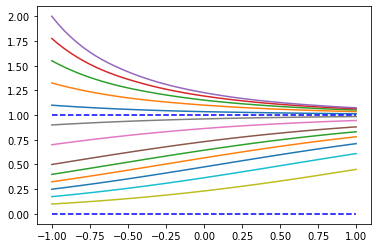
\includegraphics[scale=0.4]{sol-logistico-capa.png}\\
	Universidade Federal Fluminense\\
Instituto de Humanidades e Saúde -- RHS\\
Departamento de Ciências da Natureza -- RCN  \\
Campus de Rio das Ostras
	}
\date[{\color{orange} \today}]{ }


\frame{\titlepage}

%%%%%%%%%%%%%%%%%%%%%%%%%% sumario  %%%%%%%%%%%%%%%%%%%%%%%%%%%%%%%%

\frame{
 \frametitle{Sumário}
 \tableofcontents
}



%\AtBeginSection[]
%{
% \begin{frame}
%
%  \frametitle{Sumário}
%  \tableofcontents[currentsection]
%
% \end{frame}
%}

\section{EDO's}




\begin{frame}
\frametitle{Equa��es Diferenciais Ordin�rias }
%\begin{scriptsize}

Uma equa��o alg�brica � uma equa��o em que as inc�gnitas s�o n�meros. Uma \dt{equa��o diferencial} � uma equa��o em que as inc�gnitas s�o fun��es e a equa��o envolve derivadas desta fun��o. 

\begin{exe}
Primeiros modelos:
\begin{enumerate}
\item \textbf{Crescimento Populacional Malthusiano:} $y'=ky$ 
\item \textbf{Crescimento Populacional Log�stico:} $y'=ky(M-y)$
\item \textbf{Queda Livre de Corpos:} $h''(t)=-g$
\item \textbf{Vibra��es Mec�nicas:} $my''+ky=0$
\item \textbf{P�ndulo Simples:} $\theta''+\frac{g}{\ell}\sen\theta=0.$
\end{enumerate}
\end{exe}



%\end{scriptsize}
\end{frame}




%
%
%\begin{frame}{Vibra��es Mec�nicas}
%\begin{tikzpicture}[black!75]
%		
%		% Supporting structure
%		\fill [pattern = north west lines] (-1.5,0) rectangle ++(3,.2);
%		\draw[thick] (-1.5,0) -- ++(3,0);
%		
%		% Spring + Arrows
%		\draw[] (0,0) -- ++(0,-0.25);
%		\draw[decoration={aspect=0.3, segment length=1.2mm, amplitude=2mm,coil},decorate] (0,-0.25) -- ++(0,-2.25) node[midway,right=0.25cm,black]{{\color{red}$k$}}; 
%		\draw[] (0,-2.5) -- ++(0,-0.3) node[coordinate](c1){};
%		
%		\begin{scope}[xshift=4cm]
%			% Supporting structure
%			\fill [pattern = north west lines] (-1.5,0) rectangle ++(3,.2);
%			\draw[thick] (-1.5,0) -- ++(3,0);
%			
%			% Spring + Arrows
%			\draw[] (0,0) -- ++(0,-0.25);
%			\draw[decoration={aspect=0.3, segment length=1.4mm, amplitude=2mm,coil},decorate] (0,-0.25) -- ++(0,-2.75) node[midway,right=0.25cm,black]{{\color{red}$k$}}; 
%			\draw[] (0,-3) -- ++(0,-0.3)node[coordinate](c2){} node[draw,fill=blue!70,minimum width=1cm,minimum height=0.5cm,anchor=north,label=east:{\color{blue}$m$}](M){};
%		\end{scope}
%		
%		\begin{scope}[xshift=8cm]
%			% Supporting structure
%			\fill [pattern = north west lines] (-1.5,0) rectangle ++(3,.2);
%			\draw[thick] (-1.5,0) -- ++(3,0);
%			
%			% Spring + Arrows
%			\draw[] (0,0) -- ++(0,-0.25);
%			\draw[decoration={aspect=0.3, segment length=1.5mm, amplitude=2mm,coil},decorate] (0,-0.25) -- ++(0,-3.5) node[midway,right=0.25cm,black]{{\color{red}$k$}}; 
%			\draw[] (0,-3.75) -- ++(0,-0.3)node[coordinate](c3){} node[draw,fill=blue!70,minimum width=1cm,minimum height=0.5cm,anchor=north,label=east:{\color{blue}$m$}](M){};
%		\end{scope}
%		
%		
%		\draw[dashed,gray] (c1) -- ++(3.75,0)coordinate(c22);
%		\draw[dashed,gray] (c2) -- ++(-1.5,0) coordinate(c12);
%		\draw[latex-latex] (c12)-- (c12|-c1)node[midway,left]{\small $L$};
%
%
%		
%		\draw[dashed,gray] (c22)++(0.5,0) -- ++(3.5,0)coordinate(c33);
%		\draw[dashed,gray] (c3) -- ++(-1.5,0) coordinate(c23);
%
%	    \draw[dashed,gray] (c2)++(.5,0) -- ++(2,0) coordinate(c122);
%		\draw[latex-latex] (c122)-- (c122|-c3)node[midway,left]{\small $y$};
%		
%		
%	\end{tikzpicture}
%
%Um sistema de massa-mola composto de um corpo de massa {\color{blue}$m$} preso a uma mola, com constante el�stica {\color{red}$k$}, que est� presa ao teto satisfaz a equa��o diferencial
%\[{\color{blue}m}y''+{\color{red}k}y =0.\]
%\end{frame}
%
%
%\begin{frame}{P�ndulo Simples}
%O movimento de um p�ndulo simples de massa $m$ e comprimento $\ell$ � descrito pela fun��o $\theta(t)$ que satisfaz a equa��o diferencial
%\[\theta''+\frac{g}{\ell}\sen\theta=0.\]
%
%\end{frame}
%




\begin{frame}
\frametitle{Classifica��o }
%\begin{scriptsize}

\uncover<1->{As equa��es diferenciais s�o classificadas quanto ao \dt{tipo}, � \dt{ordem} e � \dt{linearidade}.
\begin{enumerate}[a]
\item Dizemos que uma equa��o diferencial � \dt{ordin�ria}, ou simplesmente \dt{EDO}, quando envolver somente fun��es de uma vari�vel. Caso contr�rio dizemos que � \dt{parcial}, ou simplesmente (EDP). As duas equa��es anteriores s�o EDO's e um exemplo de EDP � a seguinte equa��o
$$\frac{\partial u}{\partial x}(x,y)+\frac{\partial u}{\partial y}(x,y)=0.$$

\item Uma equa��o diferencial � dita de \dt{n-�sima ordem } quando a maior ordem das derivadas � n.

\item Uma EDO � dita \dt{linear} quando � da forma
$$a_n(t)\frac{d^ny}{dt^2}+\cdots+a_2(t)\frac{d^2y}{dt^2}+a_1(t)\frac{dy}{dt}+a_0(t)y+f(t)=0.$$
E \dt{n�o linear} caso contr�rio.

\end{enumerate} }

%\end{scriptsize}
\end{frame}



\begin{frame}
\frametitle{Solu��es de EDO's }
%\begin{scriptsize}

\uncover<1->{\begin{defin}
Uma \dt{solu��o } de uma EDO de ordem $n$ em um intervalo $I$ � uma fun��o $y(t)$ definida no intervalo $I$ tal que as derivadas at� ordem $n$ est�o definidas em $I$ e satisfazem a equa��o neste intervalo.
\end{defin} 

\begin{exe} Considere a equa��o
$$y''-3y'+2y=0.$$
Note que $y_1(t)=e^{t}$ e $y_2(t)=e^{2t}$ s�o solu��es da equa��o para todo $t\in\R$.  
\end{exe}}

%\end{scriptsize}
\end{frame}






\section{EDO's de 1\textordfeminine ordem}


\begin{frame}
\frametitle{ EDO's de 1\textordfeminine ordem}
%\begin{scriptsize}

\uncover<1->{Uma EDO de $1^{\underline{a}}$ ordem � uma equa��o da forma
$$F(t,y,y')=0.$$ 
Um problema da forma
$$\left\{\begin{array}{l}
F(t,y,y')=0\\
y(t_0)=y_0
\end{array}\right.$$
� dito \dt{problema de valor inicial (PVI)}. Uma \dt{solu��o geral} de uma EDO de $1^{\underline{a}}$ ordem, � uma fam�lia de solu��es que dependem de uma constante arbitr�ria, tal que toda solu��o particular pode ser obtida desta fam�lia por uma escolha apropriada da constante.}

%\uncover<2->{\begin{exe}
%Encontre a solu��o geral da equa��o $\frac{dy}{dt}=e^{3t}$ e uma solu��o do PVI
%$$\left\{\begin{array}{l}
%\dps\frac{dy}{dt}=e^{3t}\\
%\\
%y(1/3)=e/3.
%\end{array}\right.$$
%\end{exe} }

%\end{scriptsize}
\end{frame}


\begin{frame}{ }
	
	\begin{exampleblock}{Modelo Populacional Malthusiano}
		Este tipo de modelo � razo�vel para descrever popula��es que tem {\color{cyan}recurso ilimitados para crescimento e aus�ncia de predadores}. 
		\begin{itemize}
			\item {\color{blue}$y(t)$}: n�mero de indiv�duos de uma popula��o no instante $t$.
			\item {\color{red}$y'(t)$}: taxa de crescimento de uma popula��o no instante $t$.
			
			\item Sup�e-se que a {\color{red} taxa de crescimento} de uma popula��o � proporcional � {\color{blue} popula��o presente} 
			\[{\color{red}y'(t)}=k{\color{blue}y(t)}\]
		\end{itemize}
		
		
		\medskip
		
		Supondo que a popula��o no instante $t=0$ � $y_0$, determine a fun��o $y=y(t)$. Em quanto tempo a popula��o dobra de tamanho?
	\end{exampleblock}
\end{frame}



\begin{frame}
\begin{casa}
\begin{enumerate}
\item Determine uma solu��o geral para a equa��o
\[y'(t)=y(t).\]

\item Determine uma solu��o para o PVI
\begin{equation*}
\begin{cases}
y'=y\\
y(0)=2
\end{cases}
\end{equation*}
\end{enumerate}



\end{casa}
\end{frame}

\begin{frame}{Campos de Dire��es}
\dt{Campos de Dire��es} s�o ferramentas validas no estudo de solu��es de equa��es diferenciais da forma
\[y'(t)=f(t,y),\]
onde $f$ � uma fun��o dada chamada de \dt{fun��o taxa de varia��o}. Ele � constru�do desenhando-se em cada ponto de uma malha retangular um segmento de reta  cujo coeficiente angular � valor de $f$ naquele ponto.


\end{frame}

\begin{frame}
\begin{exe}
Campo de dire��es de $y'=y$
\begin{center}
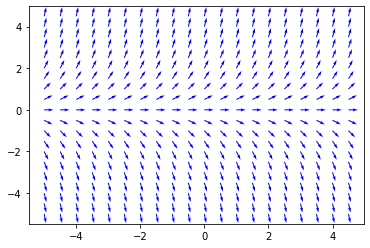
\includegraphics[scale=0.7]{CD-1.png}
\end{center}
\end{exe}
\end{frame}



\begin{frame}
\frametitle{Equa��es Separ�veis }
%\begin{scriptsize}

\uncover<1->{As EDO's de 1\fm ordem \dt{separ�veis} s�o equ��es da forma
$$g(y)\frac{dy}{dx}=f(x).$$
Integrando esta equa��o em rela��o a $x$ temos que
$$\int g(y)y'dx=\int f(x)dx+C.$$
Fazendo a substitui��o $u=y(x)$, $du=y'(x)dx$ temos que
$$\int g(u)du=\int f(x)dx+C.$$
Assim, se $G$ � uma primitiva de $g$ temos que 
$$G(y(x))=\int f(x) dx +C$$ }
%\end{scriptsize}
\end{frame}


\begin{frame}{Crescimento Populacional Log�stico}
	Vimos que um modelo simples de crescimento populacional � aquele em que se sup�e que a taxa de crescimento de uma popula��o \textcolor{blue}{$\frac{dy}{dt}$} � proporcional � popula��o presente \textcolor{blue}{$y(t)$} naquele instante.	O \dt{crescimento log�stico}, leva em conta que a popula��o tem um valor m�ximo sustent�vel \textcolor{red}{$M$}. Quando a popula��o se aproxima da capacidade m�xima, os recursos tornam-se menos abundantes e a taxa de crescimento come�a a diminuir. Uma rela��o simples  que exibe esse comportamento � quando 
	\[\textcolor{blue}{\frac{dy}{dt}}={\color{orange}k}\textcolor{blue}{y}(\textcolor{red}{M}-\textcolor{blue}{y}) \]
	
	%\begin{exe} Bi�logos colocaram em um lago 400 peixes e estimaram a capacidade de suporte como 10.000. O n�mero de peixes triplicou no primeiro ano. Encontre uma express�o para o tamanho da popula��o de peixes depois de $t$ anos.
	%\end{exe}	
	%	Usando-se o m�todo de fra��es parciais, pode-se mostrar que a popula��o � modelada por:
	%	\[{\color{blue}y(t)}=\frac{{\color{red}M}}{1+Ce^{-{\color{orange}k}{\color{red}M}t}},\ t\geq 0.\]
	%	
	
\end{frame}

\begin{frame}{ }


%\begin{minipage}{0.55\textwidth}
\begin{exe}
Considere o problema de crescimento log�stico:
	\[\begin{cases}
y'=y(1-y)\\
y(0)=y_0, y_0\geq 0.
\end{cases}
\]
Mostre que a solu��o geral � dada por:
\[y(t)=\frac{1}{1+Ce^{-t}}, t\in \R.\]
\end{exe}
%\end{minipage}
%\begin{minipage}[c]{0.4\textwidth}
%\begin{figure}
%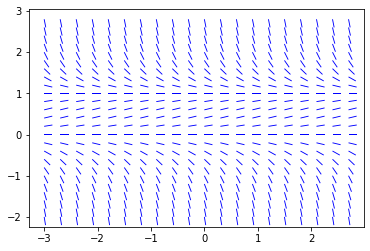
\includegraphics[scale=0.5]{CD-logistico.png}
%\caption{Campo de dire��es}
%\end{figure}
%\end{minipage}


\end{frame}

\begin{frame}
\begin{block}{Solu��o geral}
\[y(t)=\frac{1}{1+Ce^{-t}}, t\in \R.\]
\end{block}
\begin{figure}
\centering
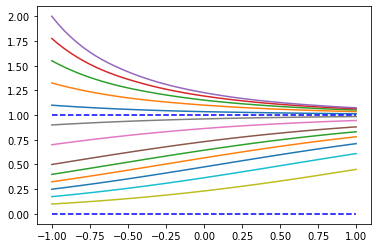
\includegraphics[scale=0.65]{sol-logistico-capa.png}
\caption{Fam�lia de Solu��es para diversos valores de $C$.}
\end{figure}
\end{frame}


\begin{frame}

\begin{exe}
\[y'=\frac{x^2}{1-y^2}\]
\end{exe}

Solu��o geral
\[y^3+x^3-3y=C\]

\begin{figure}
\centering
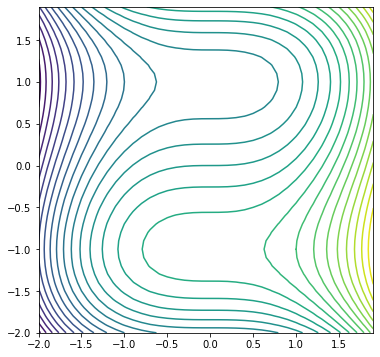
\includegraphics[scale=0.35]{sol-ex-sep.png}
\caption{Fam�lia de Solu��es para diversos valores de $C$.}
\end{figure}

\end{frame}


\begin{frame}
\frametitle{EDO's Lineares de 1\fm ordem }
%\begin{scriptsize}

As \dt{EDO's lineares de 1\fm ordem} s�o equa��es que podem ser escritas da forma
\[\frac{dy}{dt}+{\color{cyan} p(t)}y={\color{cyan} q(t)}.\]

\begin{block}{T�cnina do Fator Integrante}
Multiplicamos a equa��o por {\color{red} fator integrante} fun��o {\color{red} $\mu(t)$ }
\[{\color{red} \mu(t)} y'(t)+\only<1>{{\color{red}\mu(t)} {\color{cyan} p(t)}y}\only<2->{\underbrace{{\color{red}\mu(t)} {\color{cyan} p(t)}}_{{\color{red} \mu'(t) }}y}={\color{red}\mu(t)}{\color{cyan}q(t)}.\]

\uncover<2->{\[\Rightarrow ({\color{red} \mu(t) }y(t))'={\color{red} \mu(t) }{\color{cyan}q(t)}\]
Que pode ser resolvida por integra��o direta. O {\color{red} fator integrante} ${\color{red} \mu(t) }$ pode ser obtido por
\[{\color{red} \mu(t) }=e^{\int{\color{cyan} p(t)}dt}.\]
}

\end{block}


 
%\uncover<1->{\begin{exe} Obtenha a solu��o geral da equa��o
%$\dps y'+\frac{2}{t}y=t$ e esboce um gr�fico com as solu��es.  
%\end{exe}}


%\end{scriptsize}
\end{frame}



\begin{frame}
\begin{exe}
Determine a solu��o gerla da equa��o diferencial
\[y'+\frac{1}{2}y=\frac{1}{2}e^{t/3}.\]
Encontre a solu��o particular que passa pelo ponto $(0,1)$.
\end{exe}


\begin{center}
\only<1>{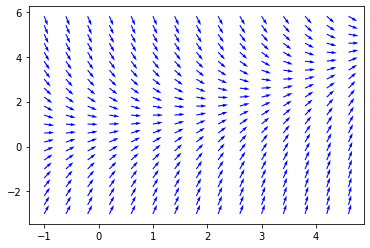
\includegraphics[scale=0.6]{CD-2.png}}
\only<2>{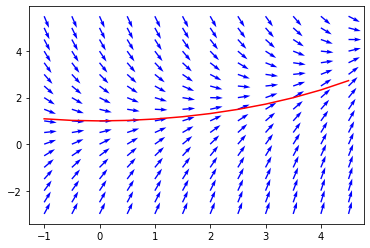
\includegraphics[scale=0.6]{CD-3.png}}
\end{center}

\end{frame}

%\begin{frame}{Queda Livre com Resist�ncia do ar}
%	Sejam um corpo de massa {\color{blue} $m$} que est� caindo e que sofre uma for�a de resist�ncia do ar que � proporcional � velocidade do corpo. Adotando-se o referencial positivo para baixo, a velocidade satisfaz a equa��o:
%	\[mv'+kv=mg\]
%	
%\end{frame}
\begin{frame}{Queda Livre com Resist�ncia do ar}
	Sejam um corpo de massa {\color{blue} $m$} que est� caindo e que sofre uma {\color{red}for�a de resist�ncia do ar que � proporcional � velocidade do corpo}. Adotando-se o referencial positivo para baixo, a velocidade satisfaz a equa��o:
\[{\color{blue}m}v'+{\color{red}k}v={\color{blue}m}g\]
	
\begin{exe} Um p�ra-quedista com o seu p�ra-quedas pesam 70 quilogramas e salta de uma altura de 1400 metros. O p�ra-quedas abre automaticamente ap�s 5 segundos de queda. Sabe-se que a velocidade limite � de 5 $m/s$. Determine a velocidade que o p�ra-quedista atinge no momento que o p�ra-quedas abre. Quanto tempo demora para a velocidade chegar a 5,1 $m/s$. Como varia a altura em fun��o do tempo?
\end{exe}
\end{frame}

\begin{frame}
\begin{casa}
\begin{enumerate}
\item Determine a solu��o geral da EDO: $y'-2y=4-t$

\item Resolva o PVI 
\[\begin{cases}
ty'+2y=4t^2\\
y(1)=2.
\end{cases}\]

\item Determine uma f�rmula geral para as solu��es da EDO: $y'+ay=g(t)$, onde $a$ � uma constante.
\end{enumerate}
\end{casa}
\end{frame}




%\begin{frame}
%\frametitle{ }
%
%
%\uncover<1->{\begin{exe} Encontre a solu��o do PVI
%$$\left\{\begin{array}{l}
%\frac{dy}{dx}=\frac{2x-1}{3y^2-3}\\
%y(1)=0
%\end{array} \right.$$
%\begin{enumerate}
%\item Determine o \dt{intervalo de validade da solu��o}, ou seja, o maior intervalo contendo $x_0=1$ para o qual a solu��o $y(x)$ e sua derivada est�o definidas.
%
%\item Determine os pontos onde a solu��o tem um m�ximo local.
%
%\item Fa�a um esbo�o do gr�fico da solu��o.
%\end{enumerate}
%\end{exe} }
%
%\end{frame}




\begin{frame}
\frametitle{ Equa��es Exatas}
%\begin{scriptsize}

Uma EDO de 1\fm\ ordem 
\[{\color{red}M(x,y)}+{\color{blue}N(x,y)}\frac{dy}{dx}=0,\]
� dita \dt{equa�ao diferencial exata} quando existe uma fun��o $\psi$ tal que 
\[\frac{\partial \psi}{\partial x}={\color{red}M} \text{ e } \frac{\partial \psi}{\partial y}={\color{blue}N}.\]
Neste caso, podemos reescrever a EDO da forma:
\[\frac{\partial \psi}{\partial x}+\frac{\partial \psi}{\partial y}\frac{dy}{dx}=0\]
Supondo que $y$ � uma fun��o de $x$, pela regra da cadeia para v�rias vari�veis, temos que
\[\frac{d}{dx}(\psi(x,y(x)))=0,\]
Logo a solu��o geral da EDO � dada implicitamente por
\[\psi(x,y(x))=C\]

%\end{scriptsize}
\end{frame}

\begin{frame}
\begin{exe}
Resolva a EDO: $2x+y^2+2xyy'=0$.
\end{exe}

\begin{teo}
Suponha que ${\color{red}M}, {\color{blue} N}, \frac{\partial {\color{red}M}}{\partial y},\frac{\partial {\color{blue} N}}{\partial x}$ s�o cont�nuas num ret�ngulo $[a,b]\times[c,d]$, ent�o a EDO
\[{\color{red}M(x,y)}+{\color{blue}N(x,y)}\frac{dy}{dx}=0\]
� exata se, e somente se, 
\[\frac{\partial \color{red}M}{\partial y }=\frac{\partial {\color{blue} N}}{\partial x}.\]
\end{teo}
\end{frame}


\begin{frame}
\begin{exe}
Verifique se as EDOs s�o exatas, em caso afirmativo, determine a solu��o
\begin{enumerate}
\item $(y\cos x+2xe^y)+(\sen x +x^2e^y-1)y'=0$

\item $(3xy+y^2)+(x^2+xy)y'=0$
\end{enumerate}

\end{exe}
\end{frame}

\begin{frame}{Fator Integrante: EDO exata}
No caso em que a EDO n�o � exata, podemos tentar torn�-la exata atrav�s de um fator integrante. Seja 
\[{\color{red}M(x,y)}+{\color{blue}N(x,y)}\frac{dy}{dx}=0,\ \text{ com } {\color{red}M_y}\neq {\color{blue}N_x}.\]
Pode-se obter um fator integrante $\mu$  que torna a EDO exata, da seguinte forma:
\begin{enumerate}
\item $P(x)=\frac{{\color{red}M_y}-{\color{blue}N_x}}{{\color{blue}N}}$ ent�o
$\mu(x)=e^{\int P(x)\,dx}$.


\item $Q(y)=\frac{{\color{blue}N_x}-{\color{red}M_y}}{{\color{red}M}}$ ent�o
$\mu(y)=e^{\int Q(y)\,dy}$.
\end{enumerate}

\begin{exe}
Determine o fator integrante que torne a seguinte EDO exata.
\[(3xy+y^2)+(x^2+xy)y'=0\]
\end{exe}
\end{frame}

\begin{frame}
\begin{casa}
 Encontre a solu��o geral das EDO's:
\begin{enumerate}

\item $(3xy+y^2)+(x^2+xy)y'=0$

\item $\frac{2y(1+x^2)}{1+2x^2}y'-\frac{2xy^2}{(1+2x^2)^2}=1$
\end{enumerate}
\end{casa}
\end{frame}
%
%\subsection{Aplica��es}
%
%\begin{frame}
%\frametitle{Din�mica Populacional }
%\begin{scriptsize}
%
%\uncover<1->{O modelo mais simples de \dt{crescimento populacional} � aquele em que se sup�e que a taxa de crescimento de uma popula��o $\frac{dy}{dt}$ � proporcional � popula��o presente $y(t)$ naquele instante . Um outro modelo, conhecido como \dt{crescimento log�stico}, leva em conta que a popula��o tem um valor m�ximo sustent�vel $y_M$. Quando a popula��o se aproxima da capacidade m�xima, os recursos tornam-se menos abundantes e a taxa de crescimento come�a a diminuir. Uma rela��o simples  que exibe esse comportamento � quando 
%$$\frac{dy}{dt}=ky(y_M-y)$$ 
%
%\begin{exe} Bi�logos colocaram em um lago 400 peixes e estimaram a capacidade de suporte como 10.000. O n�mero de peixes triplicou no primeiro ano.
%\begin{enumerate}
%\item Encontre uma express�o para o tamanho da popula��o de peixes depois de $t$ anos.
%
%\item Quanto tempo levar� para a popula��o aumentear para 5000?
%\end{enumerate}
%\end{exe}}
%
%\end{scriptsize}
%\end{frame}
%
%
%
%\begin{frame}
%\frametitle{Data��o por Carbono 14 }
%\begin{scriptsize}
%
%\uncover<1->{A propor��o de carbono 14(radioativo) em rela��o ao carbono 12 presentes nos seres vivos � constante. Quando um organismo morre a absor��o de carbono 14 cessa e a partir de ent�o o carbono 14 vai se transformando em carbono 12 a uma taxa proporcional a quantidade presente. Podemos descrever o problema de encontrar a quantidade de carbono 14 em fun��o do tempo, $y(t)$, como o problema de valor inicial
%$$\left\{\begin{array}{l}
%\frac{dy}{dt}=-ky\\
%y(0)=y_0.
%\end{array} \right.$$ 
%
%\begin{exe} Em um peda�o de madeira � encontrado $1/500$ da quantidade original de carbono 14. Sabe-se que a meia-vida do carbono 14 � 5600 anos, ou seja, que em 5600 anos metade do carbono 14 presente transformou-se em carbono 12. Qual a idade deste peda�o de madeira?
%\end{exe}}
%
%\end{scriptsize}
%\end{frame}
%
%
%
%\begin{frame}
%\frametitle{Lei de Resfriamento de Newton }
%
%
%\uncover<1->{A \dt{lei de resfriamento de Newton} diz que a taxa de varia��o da temperatura $T(t)$ de um corpo em resfriamento � proporcional � diferen�a entre a temperatura atual do corpo $T(t)$ e a temperatura constante do meio ambiente $T_m$, ou seja, a temperatura do corpo satisfaz a equa��o
%$$\frac{dT}{dt}=k(T-T_m)$$ 
%
%\begin{exe}
%
%Supopnha que um corpo humano foi encontrado em um motel a meia noite e sua temperature  era de 30\mc C. A temperatura do quarto (temperatura ambiente) era de 15\mc C (supor constante). Duas horas depois a temperatura do corpo era de  25\mc C. Encontre a hora da morte.
%
% 
%\end{exe}}
%
%
%\end{frame}
%
%
%
%
%\begin{frame}
%\frametitle{Lei de Torricelli }
%
%
%\uncover<1->{ A \dt{Lei de Torricelli} diz que a taxa com que um l�quido escoa por um orif�cio situado a uma profundidade $h$ � proporcional a $\sqrt{h}$, ou seja,
%$$\frac{dV}{dt}=k\sqrt{h}.$$
%
%\begin{exe} Um tambor cil�ndrico, de 2 metros de altura e base circular de raio 1 metro, est� cheio de �gua. Se fizermos um furo no fundo e em 30 minutos a �gua cair pela metade qual a altura $h$ em fun��o do tempo e em quanto tempo o tanque esvazia?
%\end{exe}}
%
%
%\end{frame}
%
%
%\begin{frame}
%\frametitle{Resist�ncia em Fluidos }
%
%
%\uncover<1->{ Um corpo que se desloca em um fluido sofre uma for�a de resit�ncia que � proporcional a velocidade do corpo. Assim, a velocidade, $v(t)$, de um corpo de massa $m$ � solu��o da equa��o
%$$m\frac{dv}{dt}=F-kv,$$
%onde $F$ � a for�a resultante atuando no corpo.
%
%\begin{exe} Um p�ra-quedista com o seu p�ra-quedas pesam 70 quilogramas e salta de uma altura de 1400 metros. O p�ra-quedas abre automaticamente ap�s 5 segundos de queda. Sabe-se que a velocidade limite � de 5 $m/s$. Determine a velocidade que o p�ra-quedista atinge no momento que o p�ra-quedas abre. Quanto tempo demora para a velocidade chegar a 5,1 $m/s$. Como varia a altura em fun��o do tempo?
%\end{exe}}
%
%
%\end{frame}



\begin{frame}
\frametitle{Exist�ncia e Unicidade de Solu��es  }


\uncover<1->{Ao se trabalhar com equ��es diferenciais duas perguntas s�o naturais: Um problema de valor inicial 
\[\begin{cases}
y'(t)=f(t,y)\\
y(t_0)=y_0
\end{cases}\]
sempre tem solu��o? Se sim essa solu��o � �nica? 

\begin{exe} 
%\begin{enumerate}
 O problema 
\[ \begin{cases}
y'=2\sqrt{y}\\
y(0)=0
\end{cases}\] tem infinitas solu��es! Para todo $c\geq 0$ s�o solu��es do PVI
$$y(t)=\left\{\begin{array}{ll}
(t-c)^2,& t\geq c\\
0, & t<c.
\end{array}  \right.$$
%\end{enumerate}
\end{exe} }

\end{frame}


\begin{frame}
\frametitle{Teorema de Exist�ncia e Unicidade de Solu��es para Equa��es Lineares }
\begin{teo} Considere o problema de valor inicial
\[\begin{cases}
y'+{\color{blue}p(t)}y={\color{blue}q(t)}\\
y({\color{red}t_0})=y_0.
\end{cases} \]
Se ${\color{blue}p(t)}$ e ${\color{blue}q(t)}$ s�o {\color{blue}cont�nuas} em um intervalo ${\color{red}I}$ contendo ${\color{red}t_0}$, ent�o o PVI {\color{red}tem uma �nica solu��o} em $I$.
\end{teo}
\end{frame}


\begin{frame}
\frametitle{Teorema de Exist�ncia e Unicidade de Solu��es Geral}


\uncover<1->{ \begin{teo} Considere o problema de valor inicial
\[\begin{cases}
y'(t)={\color{blue}f(t,y)}\\
y({\color{red}t_0})={\color{red}y_0}
\end{cases}\]
Se ${\color{blue}f(t,y)}$ e ${\color{blue}\dps\frac{\partial f}{\partial y}}$ s�o {\color{blue}cont�nuas} em um ret�ngulo
\[R=\{(t,x)\in \R^2; a<t<b, c<y<d \}\]
contendo ${\color{red}(t_0,y_0)}$, ent�o o PVI {\color{red}tem uma �nica solu��o} em um intervalo contendo $t_0$.
\end{teo}}

\end{frame}




\begin{frame}
\frametitle{ }


\uncover<1->{\begin{exe}
\begin{enumerate}
 \item A �nica solu��o do problema
\[\begin{cases}
y'(t)=-y^2\\
y(0)=1
\end{cases}\]
� {\color{blue}$y=\dps\frac{1}{t+1}$} definida no intervalo {\color{red}$(1,\infty)$}. Note que n�o existe uma solu��o definida em toda a reta!


\item O problema
\[\begin{cases}
y'=\sen(ty)+y^2\\
y(0)=1
\end{cases}\]
tem solu��o?

\end{enumerate}
\end{exe} }


\end{frame}



\subsection*{Números Complexos}


\begin{frame}{Introdução aos números complexos\footnotemark}
\footnotetext[1]{Veja o apêndice do livro James Stewart, Cálculo Volume 1.}

 O conjunto dos \dt{números complexos}, denotado por  $\mathbb{C}$, são formados pelos elementos da forma
\[z=a+bi,\ a,b\in \R, \text{ com }  i^2=-1,\]
onde estão definidas as operações de adição e multiplicação:
\begin{itemize}
\item $(a+bi)+(c+di)=(a+c)+(b+d)i$
\item $(a+bi)\cdot(c+di)=(ac-bd)+(ad+bc)i$
\end{itemize}

\begin{exe}
 Calcule $(-1+3i)(2-5i)$
\end{exe}

\end{frame}


\begin{frame}
O  \dt{módulo} de $z$ é definido por 
\[|z|:=\sqrt{a^2+b^2}.\] 

O \dt{Complexo Conjugado} de $z=a+bi$ é 
\[\bar{z}=a-bi.\]


\begin{block}{Propriedades}
\begin{enumerate}
\item $z\bar{z}=|z|^2$.
\item $\overline{z+w}=\bar{z}+\bar{w}$,\ \ \ \ $\overline{zw}=\bar{z}\bar{w}$\ \ \ \ e\ \ \ \ $\overline{z^n}=\bar{z}^n$

\item Se $z$ é raíz de um polinômio, então $\bar{z}$ também o é.
\end{enumerate}
\end{block}



\end{frame}

\begin{frame}
\begin{exe}
\begin{enumerate}
\item Expresse o número $\frac{-1+3i}{2+5i}$ na forma $a+bi$.

\item Encontre as raízes da equação $x^2+x+1$
\end{enumerate}
\end{exe}

\begin{teo}[Teorema Fundamental da Álgebra]
Toda equação polinômial 
\[a_nx^n+a_{n-1}x^{n-1}+\cdots a_1x+a_0=0,\]
onde $a_k\in \R$ e $n\geq 1$, tem exatamente $n$ soluções no conjunto dos números complexos.
\end{teo}
\end{frame}

\begin{frame}{Forma Polar}

\end{frame}
\section{EDO's de 2\textordfeminine ordem lineares }




\begin{frame}
\frametitle{ EDO's de 2\fm ordem lineares}

As \dt{EDO's de 2\fm ordem linear } s�o equa��es que podem ser escritas na forma
\[y''+{\color{blue}p(t)}y'+{\color{blue}q(t)}y={\color{red}f(t)}.\]

Uma EDO de 2\fm ordem linear � dita \dt{homog�nea} se ela pode ser escrita como
\begin{equation}\label{eq_hom_2}
y''+{\color{blue}p(t)}y'+{\color{blue}q(t)}y=0.
\end{equation}

\begin{exe}
\begin{enumerate}
\item EDO Linear de 2\fm ordem n�o-homog�nea: $y''+4y=e^t\sen t$

\item EDO Linear de 2\fm ordem homog�nea: $x^2y''+xy'+(x^2-1)y=0$

\item EDO n�o-Linear de 2\fm ordem: $yy''+y'=0$
\end{enumerate}
\end{exe}
\end{frame}



\begin{frame}
\frametitle{ }
\begin{teo}[Teorema de Exist�ncia e Unicidade das Solu��es]
Considere o PVI
\[
\begin{cases}
y''+{\color{blue}p(t)}y'+{\color{blue}q(t)}y={\color{blue}f(t)}\\
y({\color{red}t_0})= {\color{red}y_0},\  y'({\color{red}t_0})={\color{red}y_1}.
\end{cases}
\]

Se {\color{blue}$p(t)$, $q(t)$ e $f(t)$} s�o fun��es cont�nuas em um intervalo ${\color{red}I}$ contendo ${\color{red}t_0}$, ent�o o PVI tem {\color{blue} uma �nica solu��o definida neste intervalo}.
\end{teo}

\begin{exe} Encontre o maior intervalo no qual a solu��o do PVI certamente existe.
\[\begin{cases}
(t^2-3t)y''+ty'-(t+3)y=0\\
y(1)= 2,\  y'(1)=1.
\end{cases} 
\]


\end{exe}
\end{frame}

\subsection*{EDO's Homog�neas}

\begin{frame}{EDOs Lineares Homog�neas}

\begin{block}{Princ�pio da Superposi��o de Solu��es}
Para \dt{EDO's lineares homog�neas}, se $y_1(t)$ e $y_2(t)$ s�o solu��es da equa��o definidas em um mesmo intervalo, ent�o $$y(t)=c_1y_1(t)+c_2y_2(t)$$
tamb�m o �, para quaisquer constantes $c_1$ e $c_2$. 
\end{block}


\begin{exe}Mostre que $y_1(x)=x$ e $y_2(x)=x^3$ s�o solu��es da EDO mas n�o s�o solu��es do PVI.
\[\begin{cases}
 x^2y''-3xy'+3y=0\\
y(1)= 2,\  y'(1)=1.
\end{cases}
\]


\end{exe}


\end{frame}

\begin{frame}

\begin{casa}
Mostre que:

\begin{enumerate}
\item As fun��es  $y_1=\cos x$ e $y_2=\sen x$ s�o solu��es da EDO
$$y''+y=0$$

\item As fun��es $y_1=1+\cos x$ e $y_2=1+\sen x$ s�o solu��es da EDO
$$y''+y=1,$$
mas $y_1+y_2$ n�o �. 

\item As fun��es $y_1=x^2$ e $y_2=1$ s�o solu��es da EDO
$$y''y-xy'=0,$$
mas $y_1+y_2$ n�o �.
\end{enumerate}
\end{casa}
\end{frame}


%
%
%\begin{frame}
%\frametitle{  }
%\begin{scriptsize}
%
%\uncover<1->{ No �ltimo exemplo conhec�amos duas solu��es da EDO, mas n�o uma   solu��o do PVI. Ser� poss�vel determinar uma solu��o do PVI a partir dessas duas? E uma solu��o geral da EDO?}
%\bigskip
%
%\uncover<2->{Seja $\mathcal{S}$ o conjunto de todas as solu��es da EDO do �ltimo PVI definidas no intervalo $(0,+\infty)$. Da superposi��o de solu��es vemos que $\mathcal{S}$ � um \dt{subespa�o vetorial} do espa�o vetorial das fun��es cont�nuas definida no intervalo $(0,+\infty)$.}
%\bigskip
%
%\uncover<3-> {Defina a transforma��o 
%$$T:  \mathcal{S} \to  \R^2,\ \  \mbox{ por } \ \  T(y)=(y(1),y'(1)).  $$ 
%Note que
%\begin{itemize}
%\item $T$ � linear ( Exerc�cio);
%\item $T$ � um isomorfismo.
%\end{itemize}
%Portanto, $\dim\mathcal{S}=2$. Com isso, duas solu��es LI da EDO formam uma base de $\mathcal{S}$. Como $T(y_1)=(1,1)$ e $T(y_2)=(1,3)$ temos que $y_1$ e $y_2$ s�o LI, portanto qualquer solu��o da EDO � da forma
%$$ y(x)=c_1y_1(x)+c_2y_2(x), \forall x\in (0,+\infty)$$
%onde $c_1,c_2\in \R$.}
%
%
%\end{scriptsize}
%\end{frame}
%
%




\begin{frame}
\frametitle{ Solu��es Fundamentais }
 No �ltimo exemplo vimos que $y_1(x)=x$ e $y_2(x)=x^3$, $\forall\ x\in (0,+\infty)$ s�o solu��es da EDO $x^2y''-3xy'+3y=0$ mas n�o do PVI
\[\begin{cases}
 x^2y''-3xy'+3y=0\\
y(1)= 2,\  y'(1)=1.
\end{cases}
\]

Ser� poss�vel determinar uma solu��o do PVI a partir dessas duas? E uma solu��o geral da EDO?

\end{frame}
%
%
%\begin{frame}
%\frametitle{}
%\begin{scriptsize}
%
%\uncover<1->{ Com isso, uma solu��o geral da EDO � da forma
%\begin{equation}\label{edo1}
%y(x)=c_1x+c_2x^3, \forall x\in (0,+\infty).
%\end{equation}
%Para obtermos uma solu��o do PVI devemos determinar $c_1$ e $c_2$  tal que $T(y)=(2,1)$, ou seja,
%$$(2,1)=T(y)=c_1(1,1)+c_2(1,3)\Rightarrow \left\{\begin{array}{l}
%c_1+c_2=2\\
%c_1+3c_2=1.
%\end{array}\right.\Rightarrow c_1=\frac{5}{2} \mbox{ e } c_2=-\frac{1}{2}.$$
%Logo, a solu��o do PVI � 
%$$y(x)=\frac{5x}{2}-\frac{x^3}{2}, \forall x\in (0,+\infty).$$  }
%
%
%\end{scriptsize}
%\end{frame}


%\begin{frame}
%\frametitle{ Solu��es Fundamentais}
%\begin{scriptsize}
%
%
%
%\uncover<1->{Considere o PVI
%$$\left\{\begin{array}{l}
%y''+p(t)y'+q(t)y=0\\
%y(t_0)= a,\  y'(t_0)=b.
%\end{array} \right.$$
%Se $p(t)$ e $q(t)$ s�o cont�nuas, ent�o o procedimento do exemplo anterior pode ser aplicado.}
%\bigskip
%
%\uncover<2->{Sejam $y_1$ e $y_2$ duas solu��es quaisquer da EDO. Dado $\tilde{y}\in I$ qualquer, como $T_{\tilde{t}}$ � um isomorfismo, sabemos que $y_1$ e $y_2$ s�o LI se, e somente se, $T_{\tilde{t}}(y_1)=(y_1(\tilde{t}),y'_1(\tilde{t}))$ e $T_{\tilde{t}}(y_2)=(y_2(\tilde{t}),y'_2(\tilde{t}))$ s�o LI, ou ainda, se, e somente se, 
%$$\det\left(\begin{array}{cc}
%y_1(\tilde{t}) & y'_1(\tilde{t})\\
%y_2(\tilde{t}) & y'_2(\tilde{t})
%\end{array}\right)\neq 0$$}
%
%\end{scriptsize}
%\end{frame}
%
%
%\begin{frame}
%\frametitle{ }
%\begin{scriptsize}
%
%\uncover<1->{Se $y_1$ e $y_2$ s�o duas solu��es LI, ent�o a solu��o do PVI � da forma
%$y=c_1y_1+c_2y_2$. Das condi��es iniciais temos que
%$$
%\left\{\begin{array}{l}
% c_1y_1(t_0)+c_2y_2(t_0)=a\\
% c_1y'_1(t_0)+c_2y'_2(t_0)=b
%\end{array}\right.
%$$}
%
%\uncover<1->{Como $y_1$ e $y_2$ s�o  duas solu��es LI, ent�o  
%$$\det\left(\begin{array}{cc}
%y_1(t_0) & y_2(t_0)\\
%y'_1(t_0) & y'_2(t_0)
%\end{array}\right)\neq 0,$$
%Portanto o sistema linear possui �nica solu��o! }
%\bigskip
%
%\uncover<2->{ O �ltimo determinante � dito \dt{wronskiano} das fun��es $y_1$ e $y_2$ em $t_0$ e � denotado por $W[y_1,y_2](t_0)$. Se $y_1$ e $y_2$ s�o tais que $W[y_1,y_2](t)\neq 0$ para algum $t\in I$ dizemos que elas s�o  \dt{solu��es fundamentais}.}
%
%
%\end{scriptsize}
%\end{frame}




\begin{frame}
\frametitle{Wronskiano}
Considere o PVI
\[
\begin{cases}
y''+{\color{blue}p(t)}y'+{\color{blue}q(t)}y=0\\
y({\color{red}t_0})= {\color{red}y_0},\  y'({\color{red}t_0})={\color{red}y_1}.
\end{cases}
\]
Se ${\color{blue}p(t)}$ e ${\color{blue}q(t)}$ s�o cont�nuas, ent�o o procedimento do exemplo anterior pode ser aplicado. Dados {\color{cyan} $y_1$} e {\color{cyan} $y_2$} duas da EDO, ent�o o PVI ter� solu��o desde que 
\[W[{\color{cyan} y_1},{\color{cyan} y_2}]({\color{red}t_0})=
\det\left( \begin{array}{cc}
 {\color{cyan} y_1}({\color{red}t_0}) & {\color{cyan} y_2}({\color{red}t_0})  \\
{\color{cyan} y_1^\prime}({\color{red}t_0}) & {\color{cyan} y_2^\prime}({\color{red}t_0})
\end{array}
\right).\]
$W[{\color{cyan} y_1},{\color{cyan} y_2}]({\color{red}t_0})$ � chamado de {\color{blue} Wronskiano}. 


\end{frame}



\begin{frame}
\begin{teo}
Se {\color{cyan} $y_1$} e {\color{cyan} $y_2$} s�o solu��es da EDO 
\[y''+{\color{blue}p(t)}y'+{\color{blue}q(t)}y=0,\]
e se existe ${\color{red}t_0}$ tais que $W[{\color{cyan} y_1},{\color{cyan} y_2}]({\color{red}t_0})\neq 0$, ent�o a fam�lia de fun��es
\[y=c_1{\color{cyan} y_1}+c_2{\color{cyan} y_2},\]
incluem todas as solu��es da EDO, chamada \dt{solu��o geral} da EDO. Neste caso, {\color{cyan} $y_1$} e {\color{cyan} $y_2$} s�o ditas \dt{solu��es fundamentais}.
\end{teo}

\begin{exe}
Mostre que $y_1=t^{1/2}$ e $y_2=t^{-1}$ s�o solu��es fundamentais da EDO
\[2t^2y''+3ty'-y=0,\ t>0\]
e determine a solu��o geral.
\end{exe}
\end{frame}



%
%
%
%%
%%
%\begin{frame}{Vibra��es Mec�nicas}
%\begin{tikzpicture}[black!75]
%		
%		% Supporting structure
%		\fill [pattern = north west lines] (-1.5,0) rectangle ++(3,.2);
%		\draw[thick] (-1.5,0) -- ++(3,0);
%		
%		% Spring + Arrows
%		\draw[] (0,0) -- ++(0,-0.25);
%		\draw[decoration={aspect=0.3, segment length=1.2mm, amplitude=2mm,coil},decorate] (0,-0.25) -- ++(0,-2.25) node[midway,right=0.25cm,black]{{\color{red}$k$}}; 
%		\draw[] (0,-2.5) -- ++(0,-0.3) node[coordinate](c1){};
%		
%		\begin{scope}[xshift=4cm]
%			% Supporting structure
%			\fill [pattern = north west lines] (-1.5,0) rectangle ++(3,.2);
%			\draw[thick] (-1.5,0) -- ++(3,0);
%			
%			% Spring + Arrows
%			\draw[] (0,0) -- ++(0,-0.25);
%			\draw[decoration={aspect=0.3, segment length=1.4mm, amplitude=2mm,coil},decorate] (0,-0.25) -- ++(0,-2.75) node[midway,right=0.25cm,black]{{\color{red}$k$}}; 
%			\draw[] (0,-3) -- ++(0,-0.3)node[coordinate](c2){} node[draw,fill=blue!70,minimum width=1cm,minimum height=0.5cm,anchor=north,label=east:{\color{blue}$m$}](M){};
%		\end{scope}
%		
%		\begin{scope}[xshift=8cm]
%			% Supporting structure
%			\fill [pattern = north west lines] (-1.5,0) rectangle ++(3,.2);
%			\draw[thick] (-1.5,0) -- ++(3,0);
%			
%			% Spring + Arrows
%			\draw[] (0,0) -- ++(0,-0.25);
%			\draw[decoration={aspect=0.3, segment length=1.5mm, amplitude=2mm,coil},decorate] (0,-0.25) -- ++(0,-3.5) node[midway,right=0.25cm,black]{{\color{red}$k$}}; 
%			\draw[] (0,-3.75) -- ++(0,-0.3)node[coordinate](c3){} node[draw,fill=blue!70,minimum width=1cm,minimum height=0.5cm,anchor=north,label=east:{\color{blue}$m$}](M){};
%		\end{scope}
%		
%		
%		\draw[dashed,gray] (c1) -- ++(3.75,0)coordinate(c22);
%		\draw[dashed,gray] (c2) -- ++(-1.5,0) coordinate(c12);
%		\draw[latex-latex] (c12)-- (c12|-c1)node[midway,left]{\small $L$};
%
%
%		
%		\draw[dashed,gray] (c22)++(0.5,0) -- ++(3.5,0)coordinate(c33);
%		\draw[dashed,gray] (c3) -- ++(-1.5,0) coordinate(c23);
%
%	    \draw[dashed,gray] (c2)++(.5,0) -- ++(2,0) coordinate(c122);
%		\draw[latex-latex] (c122)-- (c122|-c3)node[midway,left]{\small $y$};
%		
%		
%	\end{tikzpicture}
%
%Um sistema de massa-mola composto de um corpo de massa {\color{blue}$m$} preso a uma mola, com constante el�stica {\color{red}$k$}, que est� presa ao teto satisfaz a equa��o diferencial
%\[{\color{blue}m}y''+{\color{red}k}y =0.\]
%\end{frame}
%
%
%\begin{frame}{P�ndulo Simples}
%O movimento de um p�ndulo simples de massa $m$ e comprimento $\ell$ � descrito pela fun��o $\theta(t)$ que satisfaz a equa��o diferencial
%\[\theta''+\frac{g}{\ell}\sen\theta=0.\]
%
%\end{frame}



\begin{frame}{Vibra��es Mec�nicas Amortecidas}
\begin{tikzpicture}[black!75]
		
		% Supporting structure
		\fill [pattern = north west lines] (-1.5,0) rectangle ++(3,.2);
		\draw[thick] (-1.5,0) -- ++(3,0);
		
		% Spring + Arrows
		\draw[] (0,0) -- ++(0,-0.25);
		\draw[decoration={aspect=0.3, segment length=1.2mm, amplitude=2mm,coil},decorate] (0,-0.25) -- ++(0,-2.25) node[midway,right=0.25cm,black]{{\color{red}$k$}}; 
		\draw[] (0,-2.5) -- ++(0,-0.3) node[coordinate](c1){};
		
		\begin{scope}[xshift=4cm]
			% Supporting structure
			\fill [pattern = north west lines] (-1.5,0) rectangle ++(3,.2);
			\draw[thick] (-1.5,0) -- ++(3,0);
			
			% Spring + Arrows
			\draw[] (0,0) -- ++(0,-0.25);
			\draw[decoration={aspect=0.3, segment length=1.4mm, amplitude=2mm,coil},decorate] (0,-0.25) -- ++(0,-2.75) node[midway,right=0.25cm,black]{{\color{red}$k$}}; 
			\draw[] (0,-3) -- ++(0,-0.3)node[coordinate](c2){} node[draw,fill=blue!70,minimum width=1cm,minimum height=0.5cm,anchor=north,label=east:{\color{blue}$m$}](M){};
		\end{scope}
		
		\begin{scope}[xshift=8cm]
			% Supporting structure
			\fill [pattern = north west lines] (-1.5,0) rectangle ++(3,.2);
			\draw[thick] (-1.5,0) -- ++(3,0);
			
			% Spring + Arrows
			\draw[] (0,0) -- ++(0,-0.25);
			\draw[decoration={aspect=0.3, segment length=1.5mm, amplitude=2mm,coil},decorate] (0,-0.25) -- ++(0,-3.5) node[midway,right=0.25cm,black]{{\color{red}$k$}}; 
			\draw[] (0,-3.75) -- ++(0,-0.3)node[coordinate](c3){} node[draw,fill=blue!70,minimum width=1cm,minimum height=0.5cm,anchor=north,label=east:{\color{blue}$m$}](M){};
		\end{scope}
		
		
		\draw[dashed,gray] (c1) -- ++(3.75,0)coordinate(c22);
		\draw[dashed,gray] (c2) -- ++(-1.5,0) coordinate(c12);
		\draw[latex-latex] (c12)-- (c12|-c1)node[midway,left]{\small $L$};


		
		\draw[dashed,gray] (c22)++(0.5,0) -- ++(3.5,0)coordinate(c33);
		\draw[dashed,gray] (c3) -- ++(-1.5,0) coordinate(c23);

	    \draw[dashed,gray] (c2)++(.5,0) -- ++(2,0) coordinate(c122);
		\draw[latex-latex] (c122)-- (c122|-c3)node[midway,left]{\small $y$};
		
		
	\end{tikzpicture}

Considere um sistema de massa-mola composto de um corpo de massa {\color{blue}$m$} preso a uma mola, com constante el�stica {\color{red}$k$}, que est� presa ao teto. Se levarmos em conta um amortecimento viscoso proporcional � velocidade do corpo, ent�o o sistema satisfaz a EDO
\[{\color{blue}m}y''+{\color{orange}\gamma} y'+{\color{red}k}y =0,\]
onde ${\color{orange}\gamma}>0$ � a constante de amortecimento.
\end{frame}


\begin{frame}
\frametitle{Equa��es homog�neas com coeficientes constantes }

Uma EDO linear de 2\fm ordem, homog�nea, com coeficientes constantes � uma equa��o  da forma
\begin{equation}\label{coef_const}
ay''+by'+cy=0,\ a,b,c\in\R,\ a\neq 0.
\end{equation} 
 
\bigskip

Para resolver uma equa��o do tipo (\ref{coef_const}) vamos nos inspirar no caso de 1\fm ordem. Uma EDO linear homog�na de 1\fm com coeficientes constantes � da forma
\[ay'+by=0,\ a,b\in\R,\ a\neq 0.\]
Sabemos que as solu��es para esta equa��o s�o $\dps y(t)=ce^{-bt/a}$. Neste caso � natural supor que uma solu��o da EDO (\ref{coef_const}) seja da forma $y(t)=e^{\lambda t}$ para alguma constante $\lambda$. Da�, substituindo em (\ref{coef_const}) temos que
\[a\lambda^2e^{\lambda t}+b\lambda e^{\lambda t}+ce^{\lambda t}=0\Leftrightarrow a\lambda^2+b\lambda+c=0.\]
A �ltima equa��o � dita \dt{equa��o caracter�stica.}

\end{frame}


\begin{frame}{Ra�zes Reais Distintas}
\begin{exe}
 Determinar a solu��o geral da EDO: $y''+y'-2y=0$.
\end{exe}

\begin{block}{}

Se $\lambda_1$ e $\lambda_2$ s�o ra�zes distintas da equa��o caracter�stica, ent�o a solu��o geral da EDO �:
\[y(t)=c_1e^{\lambda_1t}+c_2e^{\lambda_2t}, t\in \R.\]
\end{block}



\end{frame}

\begin{frame}{Ra�zes Reais Iguais}




\begin{exe}
 Determinar a solu��o geral da EDO: $y''+4y'+4y=0$
\end{exe}
\begin{block}{}
Se $\alpha$ � a �nica raiz da equa��o caracter�stica, ent�o a solu��o geral da EDO �:
\[y(t)=c_1e^{\alpha t}+c_2te^{\alpha t}, t\in \R.\]


\end{block}

\end{frame}


%\begin{frame}
%
%\begin{exe} Determinar as solu��es da equa��o:
%\begin{enumerate}[a]
%\item $y''+y'-2y=0$
%\item $y''+2y'+y=0$
%\item $y''-2y+2=0$
%\end{enumerate}
%\end{exe}
%\end{frame}

%\begin{frame}
%\frametitle{ }
%\begin{scriptsize}
%
%\uncover<1->{\begin{obs}
%
%\begin{enumerate}[a)]
%
%\item Se um dos coeficientes da EDO, $p(t)$ ou $q(t)$,  n�o �  cont�nuo no intervalo $I$, ent�o o Wronskiano pode se anular e as fun��es serem LI! De fato, se no exemplo anterior procurarmos por solu��es definidas em toda a reta, ent�o as fun��es 
%$$ y_1=x^3\ \  \mbox{ e } \ \ 
%y_2=\left\{ \begin{array}{ll}
%x^3,& x\geq 0\\
%-x^3,& x<0
%\end{array}  \right.$$
%s�o solu��es LI da EDO $y''-\frac{3}{x}y'+\frac{3}{x^2}y=0$ e $W[y_1,y_2](x)=0$ para todo $x\in \R.$ Isso ocorre pois as fun��es n�o s�o cont�nuas em nenhum intervalo contendo a origem. Entretanto, se restringirmos a intervalos que n�o cont�m a origem elas s�o LD, como por exemplo o intervalo $(-\infty,0)$, neste caso $y_1=-y_2$. Note ainda que $y_3=x$ tamb�m � solu��o da EDO linearmente independente das outras duas, portanto $\dim \mathcal{S}\geq 3$.
%
%\item Entretanto, se $W[y_1,y_2](t_0)\neq 0$ para algum $t_0\in I$, ent�o $y_1$ e $y_2$ s�o LI em $I$. De fato, se $W[y_1,y_2](t_0)\neq 0$, ent�o $T_{t_0}(y_1)$ e $T_{t_0}(y_2)$ s�o LI, da�,
%$$\alpha_1 y_1+\alpha_2y_2=0\Rightarrow \alpha_1 T_{t_0}(y_1)+\alpha_2T_{t_0}(y_2)=0\Rightarrow \alpha_1=\alpha_2=0.  $$
% 
%
%\end{enumerate} 
%
%\end{obs}}
%
%
%\end{scriptsize}
%\end{frame}

\begin{frame}{Revis�o de N�meros  Complexos\footnotemark}
\footnotetext[1]{Veja o ap�ndice do livro James Stewart, C�lculo Volume 1.}

\begin{itemize}
\item O conjunto dos \dt{n�meros complexos}, denotado por  $\mathbb{C}$, s�o formados pelos elementos da forma
\[z=a+bi,\ a,b\in \R, \text{ com }  i^2=-1,\]
onde est�o definidas as opera��es de adi��o e multiplica��o:
\begin{itemize}
\item $(a+bi)+(c+di)=(a+c)+(b+d)i$
\item $(a+bi)\cdot(c+di)=(ac-bd)+(ad+bc)i$
\end{itemize}


\item O \dt{Complexo Conjugado} de $z$ � $\bar{z}=a-bi$.


\item O  \dt{m�dulo} de $z$ � definido por $|z|:=\sqrt{a^2+b^2}$ e vale $z\bar{z}=|z|^2$.

\item Se $z$ � ra�z de um polin�mio, ent�o $\bar{z}$ tamb�m o �.
\end{itemize}

\end{frame}



\begin{frame}
Vamos estudar inicialmente o caso
\[y''+{\color{red}\beta^2}y=0,\]
cujas solu��es fundamentais s�o $y_1=e^{i{\color{red} \beta}t}$ e $y_2=e^{-i{\color{red} \beta}t}$. Mas como podemos escrev�-las na forma padr�o  $a+bi$?
\medskip

Primeiramente, note que $u_1(t)=\cos( {\color{red} \beta}t)$ e $u_2(t)=\sen( {\color{red} \beta}t)$ tamb�m s�o solu��es fundamentais da EDO. Portanto, 
\[y_1(t)=c_1\cos( {\color{red} \beta}t)+c_2\sen( {\color{red} \beta}t).\]
%Como $y_1(0)=1$ e $y_1'(0)=i{\color{red} \beta}$, da�, temos que $c_1=1$ e $c_2=i$. Logo,
%\[e^{i{\color{red}\beta}t}=\cos( {\color{red} \beta}t)+i\sen( {\color{red} \beta}t).\]
%Em particular, para $t=1$, temos que 
%\[e^{i{\color{red} \beta}}=\cos( {\color{red} \beta})+i\sen( {\color{red} \beta}).\]
\end{frame}

\begin{frame}{A exponencial complexa}
At� agora temos que
\[\begin{cases}
y_1(t)=e^{i{\color{red} \beta}t}\\
y_1(t)=c_1\cos( {\color{red} \beta}t)+c_2\sen( {\color{red} \beta}t).
\end{cases}\]
Como $y_1(0)=1$ e $y_1'(0)=i{\color{red} \beta}$, da�, temos que $c_1=1$ e $c_2=i$. Logo,
\[e^{i{\color{red} \beta}t}=\cos( {\color{red} \beta}t)+i\sen( {\color{red} \beta}t).\]
Em particular, para $t=1$, temos que 
\[e^{i{\color{red} \beta}}=\cos( {\color{red} \beta})+i\sen( {\color{red} \beta}).\]



\end{frame}


\begin{frame}
Curiosamente, quando  ${\color{red} \beta}=\pi$, obtemos {\color {red} a mais bela de todas as equa��es da matem�tica}:
\begin{block}{Equa��o de Euler}
\[e^{i\pi}+1=0.\]
\end{block}



De forma geral, obtemos:
\[e^{{\color{blue}\alpha}+{\color{red} \beta} i}=e^{\color{blue}\alpha} e^{{\color{red} \beta} i}=e^{\color{blue}\alpha}(\cos {\color{red} \beta} +i\sen {\color{red} \beta}),\]
conhecida como f�rmula de Euler.
\end{frame}


\begin{frame}{Ra�zes Complexas}
\begin{exe}
Determine a solu��o geral da EDO : $y''-4y'+13y=0$.
\end{exe}
\begin{block}{ }
Se $\lambda_1={\color{blue}\alpha}+{\color{red} \beta} i$ e $\lambda_2={\color{blue}\alpha}-{\color{red} \beta} i$, ent�o a solu��o geral da EDO �:
\[y(t)=e^{{\color{blue}\alpha} t}(c_1\cos({\color{red} \beta} t)+c_2\sen({\color{red} \beta} t)),\ t\in \R.\]
\end{block}
\end{frame}


\section{Vibra��es Mec�nicas Livres}

\subsection{Vibra��es Livres}

\begin{frame}{Vibra��es Mec�nicas Livres}
Vimos que o modelo para um sistema massa-mola preso no teto em um meio viscoso �:
\[{\color{blue}m}y''+{\color{orange}\gamma} y'+{\color{red}k}y =0,\]
onde {\color{blue}$m$} � a massa, ${\color{red}k}>0$ � a constante el�stica e   ${\color{orange}\gamma}>0$ � a constante de amortecimento.
\end{frame}

\begin{frame}{Vibra��es livres n�o-amortecidas}
Quando ${\color{orange}\gamma}=0$, o sistema n�o tem amortecimento e podemos reescrever a equa��o:
\[y''+{\color{violet}\omega_0^2}y =0,\]
onde ${\color{violet}\omega_0^2}=\frac{{\color{red}k}}{{\color{blue}m}}$. Com isso a solu��o geral �:
\[y=A\cos({\color{violet}\omega_0}t)+B\sen({\color{violet}\omega_0}t),\ t\in \R.\]
 A solu��o pode ser reescrita como:
\[y=R\cos({\color{violet}\omega_0}t-\delta),\]
onde $A=R\cos\delta$, $B=R\sen \delta$. O \dt{per�odo} do movimento � $T=\frac{2\pi}{{\color{violet}\omega_0}}$, a \dt{frequ�ncia} � $f=\frac{{\color{violet}\omega_0}}{2\pi}$, a \dt{amplitude} � $R$ e o par�metro adimensional $\delta$ � chamado de \dt{fase}.

\end{frame}


\begin{frame}
O movimento descrito � chamado \dt{movimento harm�nico}.
\begin{center}
\begin{tikzpicture}
  \begin{axis}%
    [clip mode=individual,
	 grid=both,
     minor tick num=4,
     grid style={line width=.5pt, draw=gray!10},
     major grid style={line width=.2pt,draw=gray!50},
     axis lines=middle,
	 yticklabels={,,},
	 xticklabels={,,},
     enlargelimits={abs=0.2}
	]
    \addplot[domain=0:2.6,samples=50,smooth,red,thick] {cos(deg(pi*x-0.4*pi))};
\node[left ] at (0,1) {$R$};
\node[left ] at (0,-1) {$-R$};
\node[below] at (.4,0) {$\frac{\delta}{{\color{violet}\omega_0}}$};
\draw[dashed,cyan,thick] (0.4,0) -- (0.4,1);
\node[below] at (2.4,0) {$\frac{2\pi+\delta}{{\color{violet}\omega_0}}$};
\draw[dashed,cyan,thick] (2.4,0) -- (2.4,1);
\node at (3,0) {$t$};
\node at (0,1.3) {$y$};
\node at (1.5,1.5) {$y=R\cos({\color{violet}\omega_0}t-\delta)$};
  \end{axis}
\end{tikzpicture}
\end{center}

\end{frame}

\begin{frame}
\begin{center}
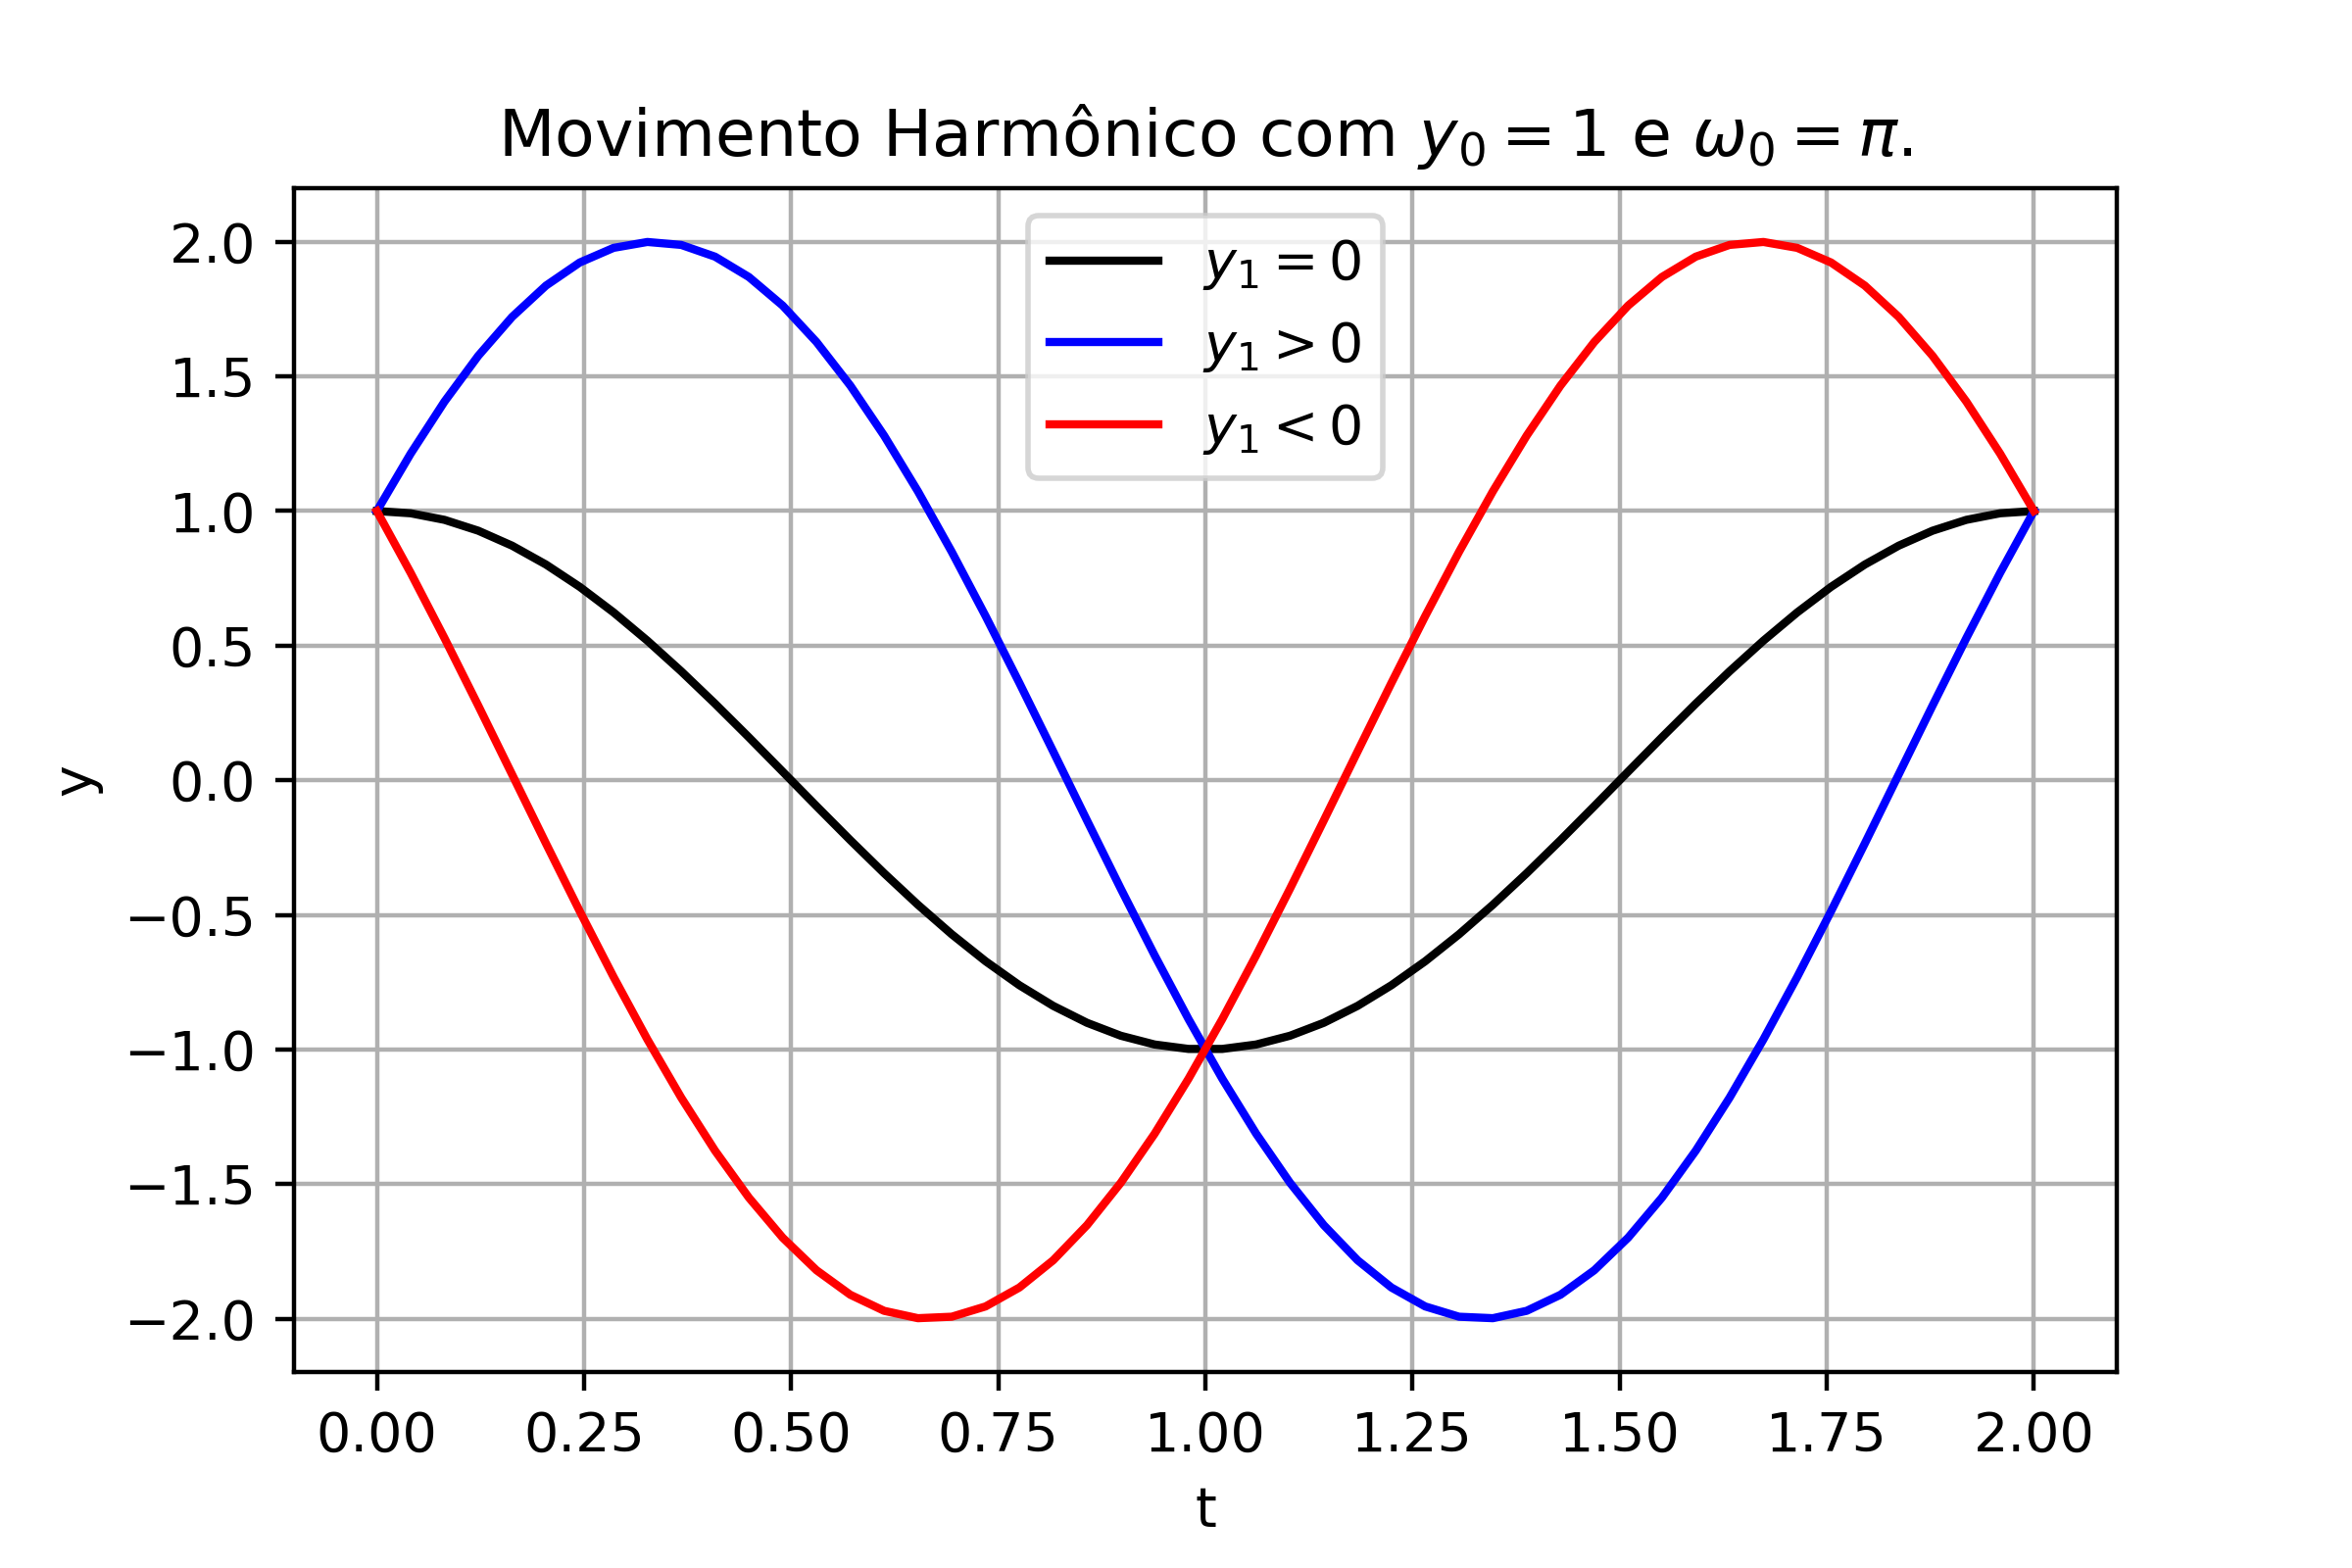
\includegraphics[scale=0.8]{osc-harm.png}
\end{center}
\end{frame}


\subsection{Vibra��es Livres Amortecidas}


\begin{frame}{Vibra��es Livres Amortecidas}
Quando o sistema � amortecido temos a equa��o:
\[{\color{blue}m}y''+{\color{orange}\gamma} y'+{\color{red}k}y =0.\]
Donde temos a equa��o caracter�stica:
\[{\color{blue}m}\lambda^2+{\color{orange}\gamma} \lambda+{\color{red}k} =0,\]
cujas ra�zes s�o:
\[\lambda=-\frac{{\color{orange}\gamma}}{2{\color{blue}m}}\pm \frac{\sqrt{{\color{orange}\gamma}^2-4{\color{blue}m} {\color{red}k}}}{2{\color{blue}m}},\]
o que nos fornece 3 casos:

\begin{enumerate}
\item \textbf{Superamortecimento}: \quad ${\color{orange}\gamma}^2>4{\color{blue}m} {\color{red}k}$
\item \textbf{Subamortecimento}: \qquad  ${\color{orange}\gamma}^2<4{\color{blue}m} {\color{red}k}$
\item \textbf{Amortecimento Cr�tico}: \ ${\color{orange}\gamma}^2=4{\color{blue}m} {\color{red}k}$
\end{enumerate}
\end{frame}


\begin{frame}{Superamortecimento}
 \[y(t)=c_1e^{\lambda_1 t}+c_2e^{\lambda_2 t},\]
onde $\lambda_1,\lambda_2<0$.

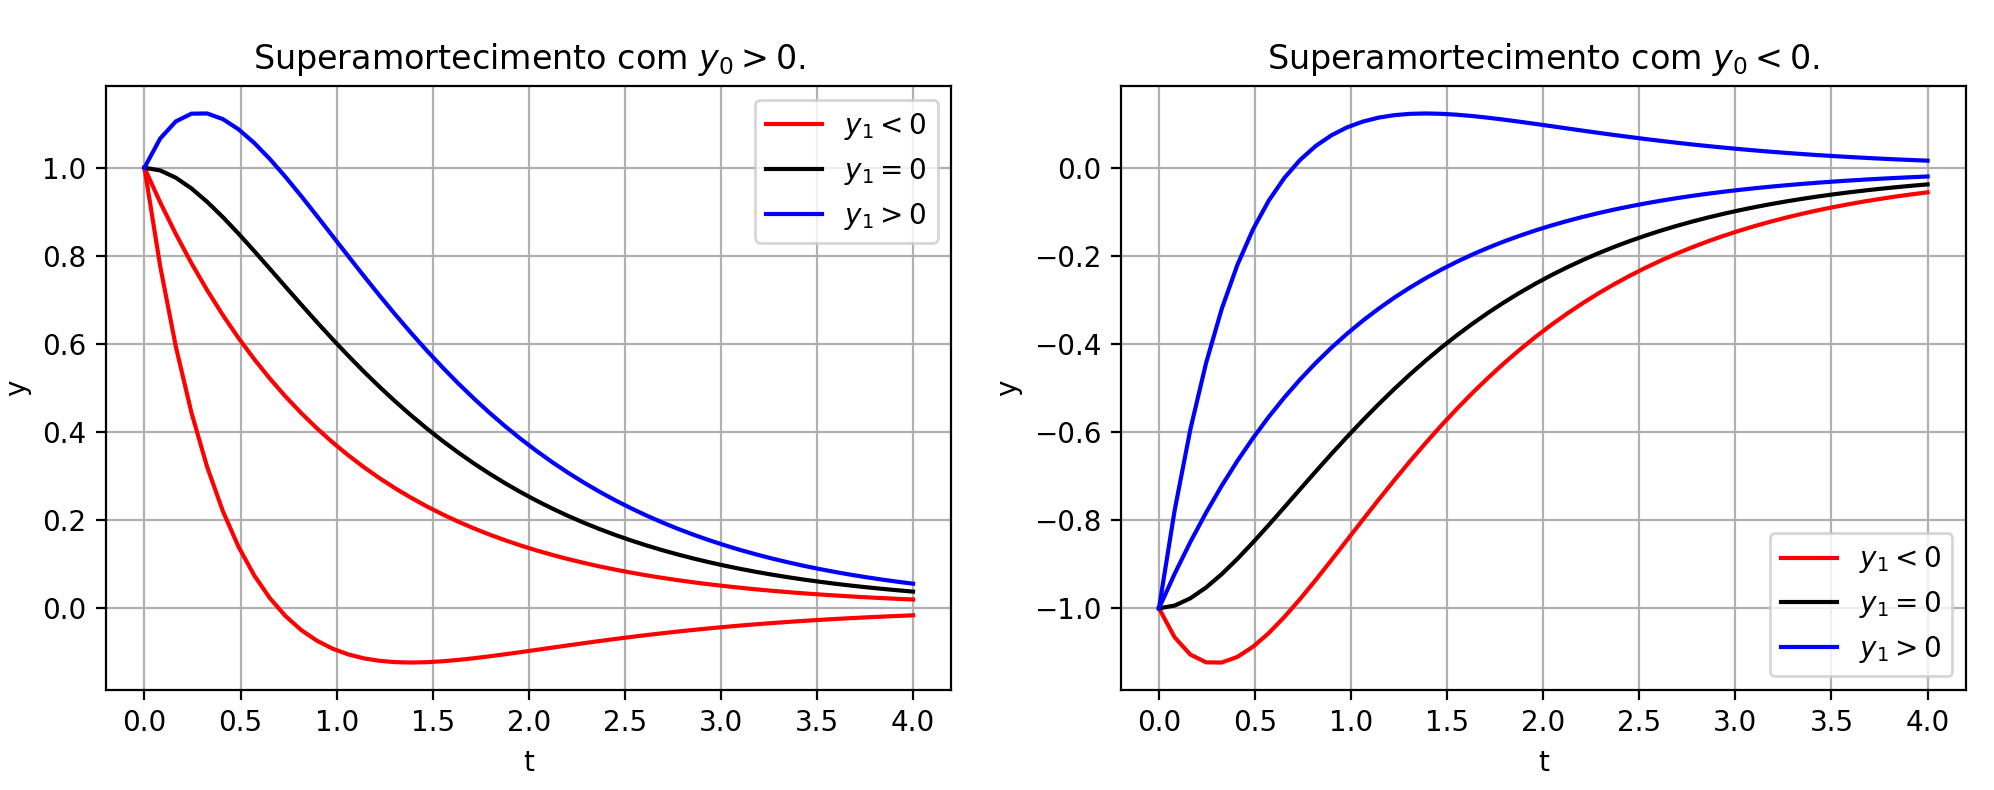
\includegraphics[scale=0.45]{osc-super.png}
%\begin{tikzpicture}
%%	\def\m{1}
%%	\def\k{2*\m}
%%	\def\g{3*\m}
%%\def\a{\g/(2*\m)}
%%\def\b{sqrt(\g*\g-4*\m*\k)/(2*\m)}
%%\def\L{-\a+\b}
%%\def\l{-\a-\b}
%  \begin{axis}%
%    [clip mode=individual,
%	 grid=both,
%     minor tick num=4,
%     grid style={line width=.5pt, draw=gray!10},
%     major grid style={line width=.2pt,draw=gray!50},
%     axis lines=middle,
%	 %yticklabels={,,},
%	 %xticklabels={,,},
%     enlargelimits={abs=0.2}
%	]
%    \addplot[domain=0:4,samples=50,smooth,red,thick] {2.7*exp(-\x)-2.1*exp(-2*\x)};
%	\addplot[domain=0:4,samples=50,smooth,cyan,thick] {0.4*exp(-\x)+0.1*exp(-2*\x)};
%	\addplot[domain=0:4,samples=50,smooth,orange,thick] {-3.3*exp(-\x)+3*exp(-2*\x)};
%%\node[left ] at (0,1) {$R$};
%%\node[left ] at (0,-1) {$-R$};
%%\node[below] at (.4,0) {$\frac{\delta}{{\color{violet}\omega_0}}$};
%%\draw[dashed,cyan,thick] (0.4,0) -- (0.4,1);
%%\node[below] at (2.4,0) {$\frac{2\pi+\delta}{{\color{violet}\omega_0}}$};
%%\draw[dashed,cyan,thick] (2.4,0) -- (2.4,1);
%%\node at (3,0) {$t$};
%%\node at (0,1.3) {$y$};
%%\node at (1.5,1.5) {$y=R\cos({\color{violet}\omega_0}t-\delta)$};
%  \end{axis}
%\end{tikzpicture}


\end{frame}


\begin{frame}{Subamortecimento}
A solu��o � da forma
 \[y(t)=e^{-\frac{{\color{orange}\gamma}t}{2{\color{blue}m}}}(A\cos(\mu t)+B\sen(\mu t)),\]
onde $\mu=\frac{\sqrt{4{\color{blue}m {\color{red}k}}-{\color{orange}\gamma}^2}}{2{\color{blue}m}}$.
Que pode ser reescrita como
 \[y(t)=Re^{-\frac{{\color{orange}\gamma}t}{2{\color{blue}m}}}\cos(\mu t-\delta),\]
onde $A=R\cos\delta$ e $B=R\sen\delta$.

\begin{center}
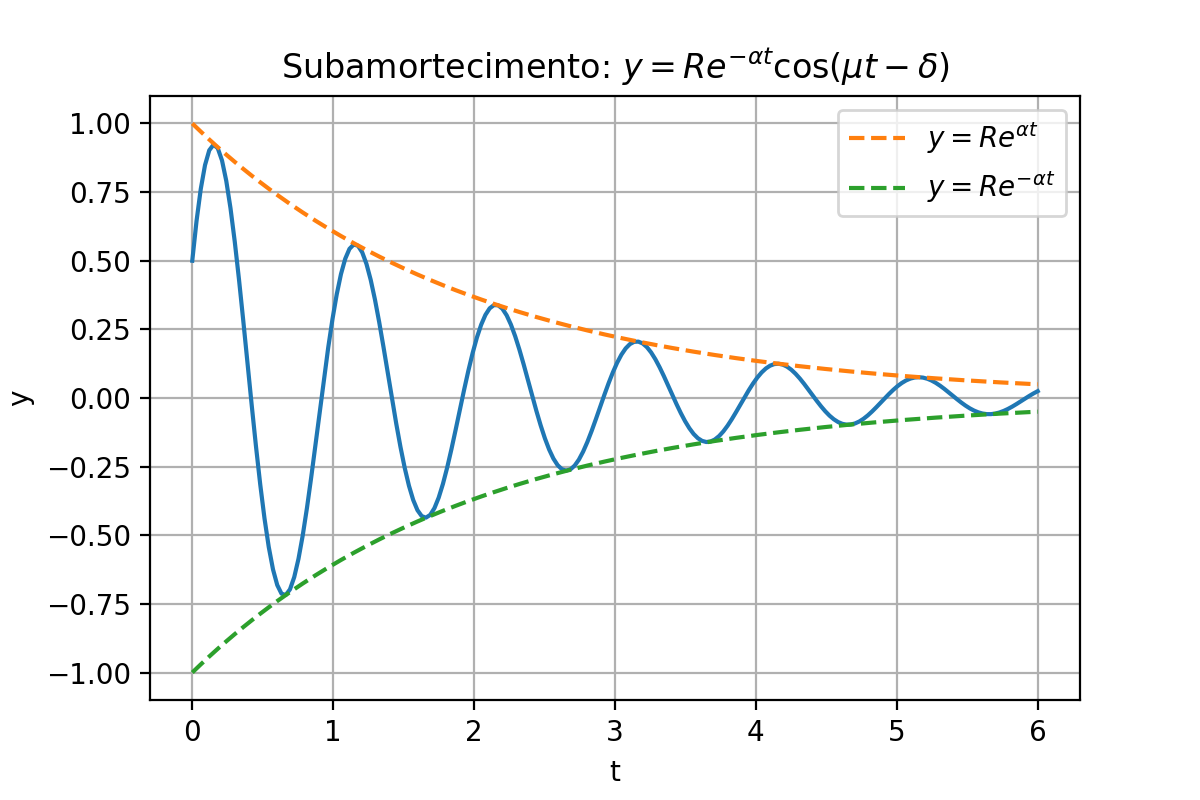
\includegraphics[scale=0.45]{osc-subarm.png}
\end{center}
\end{frame}




\begin{frame}{Amortecimento cr�tico}
A solu��o � da forma
 \[y(t)=(A+Bt)e^{-\frac{{\color{orange}\gamma}t}{2{\color{blue}m}}}.\]


\begin{center}
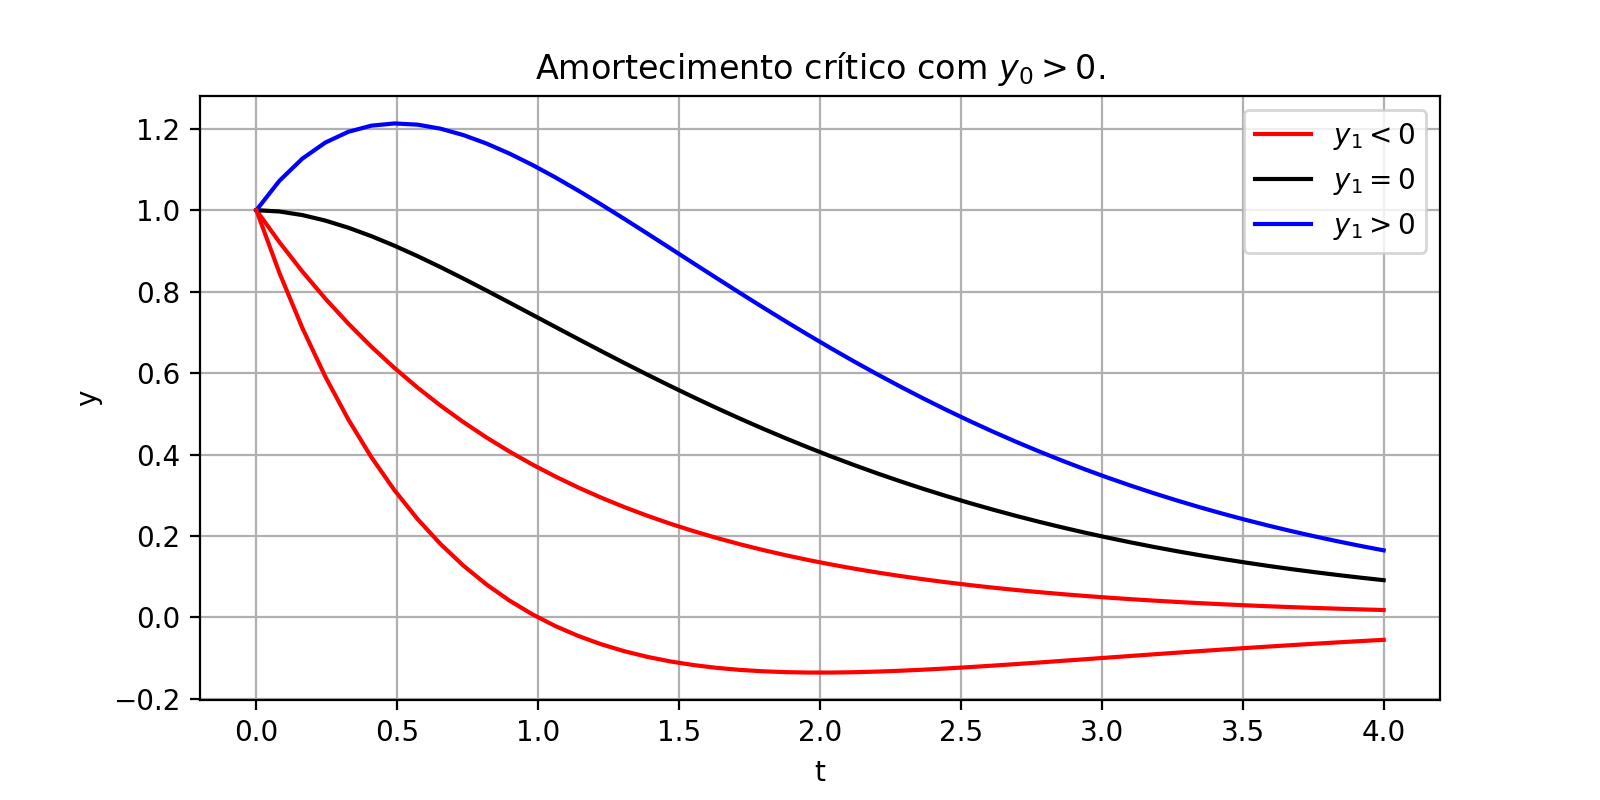
\includegraphics[scale=0.5]{osc-critico.png}
\end{center}
\end{frame}

\begin{frame}
\begin{casa}
Esboce os gr�ficos das solu��es dos problemas abaixo.
\begin{enumerate}
\item Suponha que uma massa de 4,5 kg estica uma mola x5cm. A massa � deslocada  2,5 cm para baixo e depois colocada em movimento  com uma velocidade inicial de apontando para cima de 30 cm/s. 

\item Uma massa de 20g estica uma mola 5 cm. Suponha que a massa tamb�m est� presa a um amortecedor viscoso com uma constante de amortecimento de 400 dinas$\cdot$s/cm e que a massa � puxada pra baixo mais 2 cm de depois � solta. 
\end{enumerate}
\end{casa}
\end{frame}

%
%\begin{frame}
%\frametitle{ }
%\begin{scriptsize}
%
%\uncover<1->{\begin{exe} Mostre que $y_1(t)=\cos bt$ e $y_2(t)=\sen bt$ s�o solu��es fundamentais da equa��o
%$$y''+b^2y=0$$
%
%\end{exe} }
%
%Usando o exemplo anterior podemos estender a fun��o exponencial para os n�meros complexos. Queremos definir $y(t)=e^{zt}$ para n�meros complexos $z=a+bi$ de forma que satisfa�a as propriedades
%\begin{align*}
%& e^{(a+ib)t}=e^{at}e^{ibt}\\
%& \frac{d}{dt}(e^{zt})=ze^{zt}.
%\end{align*}
%Note que a fun��o $w(t)=e^{ibt}$ � solu��o do PVI
% $$\left\{\begin{array}{l}
% y''+b^2y=0 \\
% y(0)=1,\  y'(0)=ib.
% 
%\end{array}  \right.$$
%Assim, do exemplo anterior, como $y_1(t)=\cos bt$ e $y_2(t)=\sen bt$ s�o solu��es fundamentais da EDO, temos que
%$$z(t)=\cos bt+i\sen bt.$$
%
%
%
%\end{scriptsize}
%\end{frame}
%
%
%
%\begin{frame}
%\frametitle{ }
%\begin{scriptsize}
%
%\uncover<1->{ Portanto, das propriedades de exponencial, obtemos que
%$$e^{a+bi}=z(1)=e^a(\cos b+i\sen b),$$
%conhecida como \dt{f�rmula de Euler}.}
%
%\end{scriptsize}
%\end{frame}
%
%
%\begin{frame}
%\frametitle{Equa��es homog�neas com coeficientes constantes }
%\begin{scriptsize}
%
%\uncover<1->{Uma EDO linear de 2\fm ordem, homog�nea, com coeficientes constantes � uma equa��o  da forma
%\begin{equation}\label{coef_const}
%ay''+by'+cy=0,\ a,b,c\in\R,\ a\neq 0.
%\end{equation} 
% }
%\bigskip
%
%\uncover<2->{Para resolver uma equa��o do tipo (\ref{coef_const}) vamos nos inspirar no caso de 1\fm ordem. Uma EDO linear homog�na de 1\fm com coeficientes constantes � da forma
%$$ay'+by=0,\ a,b\in\R,\ a\neq 0.$$
%Sabemos que as solu��es para esta equa��o s�o $\dps y(t)=ce^{bt/a}$. Neste caso � natural supor que uma solu��o da EDO (\ref{coef_const}) seja da forma $y(t)=e^{\lambda t}$ para alguma constante $\lambda$. Da�, substituindo em (\ref{coef_const}) temos que
%$$a\lambda^2e^{\lambda t}+b\lambda e^{\lambda t}+ce^{\lambda t}=0\Leftrightarrow a\lambda^2+b\lambda+c=0.$$
%A �ltima equa��o � dita \dt{equa��o caracter�stica.}}
%
%\uncover<3->{\begin{exe} Determinar as solu��es da equa��o:
%\begin{enumerate}[a)]
%\item $y''+y'-2y=0$
%\item $y''+2y'+y=0$
%\item $y''-2y+2=0$
%\end{enumerate}
%\end{exe}}

%
%\end{scriptsize}
%\end{frame}

\subsection*{EDO's N�o-Homog�neas}



\begin{frame}
\frametitle{Equa��es n�o-homog�neas }
%\begin{scriptsize}

� f�cil ver que se {\color{red}$y_p(t)$} � uma solu��o de uma EDO n�o-homog�nea
\[y''+{\color{blue}p(t)}y'+{\color{blue}q(t)}y={\color{blue}f(t)},\]
 {\color{cyan}$y_1$} e {\color{cyan}$y_2$} s�o solu��es fundamentais da EDO homog�nea correspondente, ent�o a solu��o geral da equa��o n�o-homog�nea �
\[y(t)={\color{red}y_p(t)}+c_1{\color{cyan}y_1(t)}+c_2{\color{cyan}y_2(t)}.\]



\end{frame}

\begin{frame}
\begin{exe}
Se no modelo de vibra��es mec�nicas existir uma for�a externa $F=F(t)$, ent�o teremos um problema de \dt{oscila��o for�ada} que � modelado pela  seguinte equa��o n�o-homog�nea:
\[{\color{blue}m}y''+{\color{orange}\gamma} y'+{\color{red}k}y =F(t).\]

Neste caso, como determinar a solu��o do  seguinte problema  cuja for�a externa � peri�dica?
\[y''+2y'+y=2\cos(t).\]
\end{exe}
\end{frame}

\begin{frame}
\begin{center}
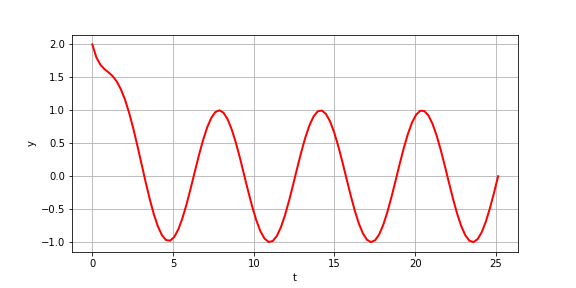
\includegraphics[scale=0.5]{osc-for-ex1.png}
\end{center}
\end{frame}




\begin{frame}
\frametitle{M�todo dos Coeficientes a Determinar }

\uncover<1->{Este m�todo funciona para qualquer EDO n�o-homog�nea com coeficientes constantes
\[ay''+by'+cy=F_1(t)+F_2(t)+\cdots+F_k(t),\]
onde  
\[F_i(t)=e^{{\color{blue}\alpha }t}[(a_0+\ldots+a_nt^{{\color{teal}n}}) \cos({\color{red}\beta}t)+(b_0+\ldots+b_mt^{{\color{teal}m}})\sen({\color{red}\beta} t)].\]

Neste caso, deve-se procurar, para cada $F_i$, uma solu��o particular da forma
\[y_p(t)=t^{{\color{cyan}s}}e^{{\color{blue}\alpha } t}[(A_0+\ldots+A_qt^{\color{teal}q})\cos({\color{red}\beta} t)+(B_0+\ldots+B_qt^{{\color{teal}q}})\sen({\color{red}\beta} t)],\]
em que ${\color{teal}q}=\max\{{\color{teal}n},{\color{teal}m}\}$,  ${\color{cyan}s}$ � o menor inteiro n�o-negativo que garante que  nenhuma parcela de $y_p$ seja solu��o da equa��o homog�nea correspondente e $A_0,\ldots,A_q,B_0,\ldots,B_q$ s�o coeficientes a serem determinados. 



}

\end{frame}

\begin{frame}
\begin{exe} Encontre a solu��o geral das seguintes equa��es:
\begin{enumerate}[a]
\item $y''+y'=2+t^2$.
\item $y''-2y'+y=e^{t}+t$
\item $y''+4y=e^t\cos t$

\end{enumerate}
\end{exe}
\end{frame}


\begin{frame}{Vibra��es Mec�nicas For�adas}
conte�do...
\end{frame}



\begin{frame}
\frametitle{ M�todo da Varia��o dos Par�metros}
%\begin{scriptsize}

Este m�todo funciona para qualquer EDO linear de 2\fm ordem 
\[y''+{\color{blue}p(t)}y'+{\color{blue}q(t)}y={\color{blue}f(t)},\]
para o qual se conhe�a duas solu��es fundamentais da equa��o homog�nea correspondente em um intervalo $I$ onde o wronskiano � n�o nulo.
\bigskip

Sabemos que a solu��o geral da equa��o homog�nea correspondente �
$$y(t)={\color{red}c_1}y_1(t)+{\color{red}c_2}y_2(t).$$
O m�todo da varia��o dos par�metros consiste em procurar uma solu��o particular da EDO n�o homog�nea que tenha  a forma da solu��o geral da homog�nea, mas substituindo os par�metros $c_1$ e $c_2$ por fun��es a determinar $u_1(t)$ e $u_2(t)$, respectivamente, ou seja, da forma
\[y(t)={\color{red}u_1(t)}y_1(t)+{\color{red}u_2(t)}y_2(t),\]
com a condi��o de que
\[{\color{red}u'_1(t)}y_1(t)+{\color{red}u'_2(t)}y_2(t)=0\]

%\end{scriptsize}
\end{frame}

\begin{frame}{F�rmula Geral}
Resolvendo-se o sistema anterior, chega-se a:
\[{\color{red}u_1(t)=-\int \frac{y_2(t)f(t)}{W[y_1,y_2](t)}\,dt,\ \text{ e } u_2(t)=\int \frac{y_1(t)f(t)}{W[y_1,y_2](t)}\,dt}\]
\begin{exe}
 Encontre a solu��o do PVI
 $$\left\{
 \begin{array}{l}
 y''+y=\sec t\\
 \\
 y(0)=1,\ y'(0)=-2.
 \end{array}\right.$$
 \end{exe} 
\end{frame}


\begin{frame}
\frametitle{ }
\begin{exe} 

\begin{enumerate}
\item Determine a solu��o geral das EDO 
\[y''+2y'+2y=\frac{e^{-x}}{\cos^3(x)}.\]
\item Verifique que $y_1(t)=t^2$ e $y_2(t)=t^{-1}$ s�o solu��es fundamentais da EDO no intervalo $(0,\infty)$
\[t^2y''-2y=3t^2-1\]
e determine a sou��o geral.
\end{enumerate}
\end{exe}
%\end{scriptsize}
\end{frame}



%
%
%\begin{frame}
%\frametitle{ }
%
%
%\center{\Huge{FIM !!!}
%\bigskip
%
%
\includegraphics[scale=0.4]{ming.eps}}
%
%\end{frame}







\end{document}



